
\section{Ejercicio 5: Distorsi\'on}
En esta secci\'on se propone el dise\~no de un sistema de distorsi\'on, donde para una se\~nal de entrada se obtenga una salida
con un efecto de saturaci\'on caracter\'istico de los pedales de efecto de distorsi\'on para guitarras el\'ectricas. Para lo cual,
se requiere que dicho dise\~no pueda alimentarse con una bateria de $9V$, incluya conectores mono de entrada y salida, y que pueda funcionar para un rango
de frecuencias de audio.

\subsection{Introducci\'on te\'orica}
En t\'erminos generales, dada una se\~nal senoidal a la cual se puede caracterizar mediante los par\'ametros de amplitud, frecuencia y fase,
y si se considera una se\~nal m\'as compleja que se puede describir a trav\'es de una serie de Fourier, como suma de senoidales de frecuencias arm\'onicas. Luego, 
se pueden aplicar diferentes tipos de transformaciones sobre tales senoidales en cualquiera de sus par\'ametros tal
que cuando las modificaciones sean lineales o no lineales pero de forma diferente para cada arm\'onico, luego tal proceso se denomina Distorsi\'on.

En particular, el an\'alisis te\'orico a realizar a continuaci\'on emplea una distorsi\'on no lineal que produce saturaci\'on en los arm\'onicos.

\subsection{An\'alisis te\'orico}
El circuito que se analizar\'a te\'oricamente est\'a compuesto de diferentes etapas que cumplen con funciones
espec\'ificas, y que bajo ciertas condiciones, se pueden analizar de forma independiente entre s\'i para simplificar el an\'alisis propuesto.

\paragraph*{Etapa Alimentaci\'on:} el circuito de alimentaci\'on, como se puede observar en la figura \ref{fig:circuito_alimentacion}
est\'a compuesto por la bateria de alimentaci\'on, una llave de encendido, y luego un diodo schottky $1N5819$ que fue colocado a modo de protecci\'on
para evitar da\~nar el circuito en caso de conexi\'on de la bateria en una polaridad opuesta. Este diodo de protecci\'on impide la circulaci\'on de corriente
en el sentido opuesto, y se utiliza el tipo de diodo Schottky porque por estar construido con una juntura metal semiconductor posee una baja tensi\'on de polarizaci\'on
lo cual implica p\'erdidas bajas en la alimentaci\'on del circuito respecto de la bateria. Adem\'as, esta baja tensi\'on de polarizaci\'on y las peque\~nas corrientes har\'an que
el diodo disipe menor potencia que si fuera un diodo rectificador com\'un.

Por otro lado, se agrega un capacitor en paralelo al diodo para compensar las variaciones de tensi\'on de entrada sin importar de donde provenga la alimentaci\'on externa. Y por \'ultimo,
se coloca un diodo led con una resistencia en serie a modo de indicador de que el circuito se encuentra en funcionamiento. Partiendo de que para corrientes bajas el diodo schottky tendr\'a
una tensi\'on $VD_{ON} \approx 0,4V$, considerando un diodo led est\'andar con $V_{LED} = 1,8$ m\'inima y que la corriente m\'axima es $I_{LED} = 20mA$, entonces:

\begin{equation}
    R_1 > \frac{9V - 0,4V - 1,8V}{20mA}
    \Rightarrow R_1 = 1k \Omega
\end{equation}

\begin{figure}[H]
    \centering
    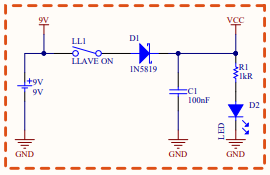
\includegraphics[]{../EJ5/Recursos/circuito_alimentacion.PNG}
    \caption{Circuito de alimentaci\'on del pedal}
    \label{fig:circuito_alimentacion}
\end{figure}

\paragraph*{Etapa Offset:} esta etapa es en la cual entra la se\~nal de entrada, la cual a priori podr\'ia tener su propio nivel de continua
del cual se requiere proteger al circuito porque luego se busca agregar un nivel de continua de $4,5 V$ ya que de esa forma se puede emplear
una etapa de amplificaci\'on con amplificador operacional sin utilizar una fuente partida. Por ende, la funci\'on de cada componente en esta etapa
desde un punto de vista cualitativo es que, el capacitor $C_2$ bloquea la componente de corriente continua de la se\~nal de entrada externa, luego las resistencias
$R_4$ y $R_5$ buscan agregar el offset de continua mencionado antes, y finalmente la resistencia $R_3$ provee una malla cerrada a trav\'es de la cual el capacitor puede
circular corriente para descargarse, adem\'as de incidir en la impedancia de entrada del circuito.

\begin{figure}[H]
    \centering
    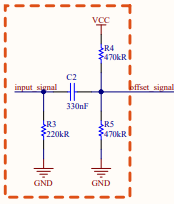
\includegraphics[]{../EJ5/Recursos/circuito_offset.PNG}
    \caption{Circuito etapa de offset del pedal}
    \label{fig:circuito_offset}
\end{figure}

Para el an\'alisis cuantitativo, por ser un sistema compuesto por componentes lineales cuando se alcanza el r\'egimen permanente, luego se aplica
principio de superposici\'on y se analiza el efecto de la parte de continua y alterna sobre la se\~nal de salida de esta etapa. Consid\'erese $V_i$ y $V_o$ la entrada y salida, respectivamente,
de dicha etapa. En primer lugar, el efecto de la continua imponiendo que se quiere $V_o = \frac{V_{CC}}{2}$ da como resultado que:

\begin{equation}
    V_o = \frac{V_{CC} \cdot R_5}{R_4 + R_5} = \frac{V_{CC}}{2} 
    \Rightarrow
    R_4 = R_5
    \label{eq:divisor_tension}
\end{equation}

Luego, desde el efecto de la alterna, si llamamos $R_p = R_4 // R_5 = \frac{R_4 \cdot R_5}{R_4 + R_5}$, entonces la transferencia del sistema
la define un divisor de tensi\'on compuesto por la $R_p$ y la $C_2$.

\begin{equation*}
    V_o = V_i \cdot \frac{R_p}{R_p + \frac{1}{s \cdot C_2}}
    \Rightarrow
    H(s) = \frac{V_o}{V_i} = \frac{s \cdot R_p \cdot C_2}{1 + s \cdot C_2 \cdot R_p}
\end{equation*}

Asumiendo un sistema LTI, causal y bibo-estable, se puede observar que el sistema se comporta como un filtro pasaaltos, donde
la frecuencia de corte est\'a ubicada en $f_o = \frac{1}{2 \pi \cdot C_2 \cdot R_p}$ y considerando que antes se llego a que las resistencias
$R_4 = R_5$, entonces $R_p = \frac{R_4}{2}$. Se impone que la frecuencia de corte se encuentre de forma tal que la fase ya sea $0^{\circ}$ para 
la espectro audible, por lo cual se pide que $10 \cdot f_o = 20Hz$ y se obtiene que:

\begin{equation}
    C_2 = \frac{1}{2 \pi \cdot R_4}
    \label{eq:capa_offset}
\end{equation}

Finalmente, para imponer condiciones sobre $R_3$ se propone analizar la impedancia de entrada del circuito. En este punto, se necesita suponer
que aquellas etapas que vengan despu\'es de esta no implican una carga significativa y se desprecian las corrientes que se vayan por $V_o$.

\begin{equation*}
    Z_{in} = \frac{V_i}{I_i} = R_3 // \left( \frac{1}{s \cdot C_2} + \frac{R_4}{2} \right)
    \Rightarrow
    Z_{in} = R_3 \cdot \frac{1+ s \cdot \frac{C_2 \cdot R_4}{2}}{1 + s \cdot \frac{C_2 \cdot (R_4 + R_3 \cdot 2)}{2}}
\end{equation*}

Analizando la respuesta en frecuencia del resultado obtenido, se puede ver que hay un polo y un cero, donde la frecuencia del polo es m\'as chica que la del cero,
y adem\'as este cero se encuentra ubicado en la misma frecuencia de corte que el filtro pasaaltos analizado con anterioridad. En conclusi\'on, para las frecuencias del rango
audible que se esperan que entren al circuito y pasen por el filtro, la impedancia de entrada se mantiene invariante en frecuencia y su valor se puede calcular considerando
que $f >> f_o = \frac{1}{2 \pi \cdot C_2 \cdot R_p}$. Entonces:

\begin{align*}
    & |Z_{in}| \rightarrow \frac{R_4 \cdot R_3}{R_4 + 2 \cdot R_3} = \frac{1}{2} \cdot \frac{R_3 \cdot R_4}{R_3 + \frac{R_4}{2}} \\
    & \Rightarrow |Z_{in}| \rightarrow R_p // R_3
\end{align*}

De esta \'ultima expresi\'on se puede ver que el valor \'optimo para la impedancia de entrada del circuito, es decir donde su valor
sea el m\'as grande posible, es cuando se cumple que:

\begin{equation}
    R_3 = R_p \Rightarrow R_3 = \frac{R_4}{2}
\end{equation}

Finalmente, s\'olo es necesario definir un valor de $R_4$ y a partir de este mismo, se obtienen como resultado los dem\'as para cumplir con los criterios tomados. Para definir su valor,
se tiene en cuenta que no se puede emplear un valor muy grande ya que se convierte en una fuente de ruido, ni muy peque\~no para que no haya un consumo de corriente elevado. Con lo cual se opt\'o por utilizar
un valor de $R_4 = R_5 = 470k \Omega$. Entonces se necesitan $C_2 = 338,62nF \approx 330nF$ y $R_3 = 235k \Omega \approx 220k \Omega$.

\paragraph*{Etapa Amplificaci\'on:} en esta etapa el objetivo es amplificar la componente alterna de la se\~nal de entrada, sin amplificar o modificar la componente de continua
de $4,5V$, puesto que se desea que la se\~nal de salida tenga suficiente amplitud que sea apreciable a los valores de polarizaci\'on de los diodos que vendr\'an en la etapa posteriormente.
En el circuito, $R_6$, $R_7$ y $R_8$ definen la realimentaci\'on y ganancia del amplificador, pero tambi\'en afectan a la ubicaci\'on del o los polos del sistema de esta etapa,
ya que el capacitor $C_3$ deber\'a corresponderse con un circuito abierto para las corrientes continuas, para las cuales la etapa tendr\'a una ganancia unitaria.

\begin{figure}[H]
    \centering
    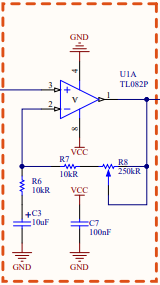
\includegraphics[]{../EJ5/Recursos/circuito_amplificador.PNG}
    \caption{Circuito de amplificaci\'on del pedal}
    \label{fig:circuito_amplificador}
\end{figure}

Para el dise\~no de esta etapa se propone hacer un an\'alisis del amplificador operacional teniendo en cuenta
un $A_{vol}$ finito, donde luego se desarrolla planteando un conjunto de aproximaciones que idealizan el comportamiento del circuito
para simplificar el c\'alculo de la etapa. Finalmente, se establecen condiciones para determinar c\'omo deben ser las caracter\'isticas del amplificador
operacional para que tales aproximaciones sean v\'alidas y en funci\'on de ello realizar la selecci\'on del mismo, de forma tal
que se pueda garantizar el correcto funcionamiento de la etapa. Sean $V_i$ y $V_o$ las respectivas entrada y salida de esta etapa, se analiza sin considerar el efecto de $R_8$ entonces:

\begin{align*}
    V^{-} &= V_i \\
    V^{+} &= V_o \cdot \frac{1 + s \cdot C_3 \cdot R_6}{1 + s \cdot C_3 \cdot (R_6 + R_7)} \\
    V_o &= (V^{+} - V^{-}) \cdot A_{vol}
\end{align*}

\begin{equation}
    H(s) = \frac{V_o}{V_i} = \frac{A_{vol}}{1 + A_{vol}}\frac{1 + s \cdot C_3 \cdot (R_6 + R_7)}{1 + s \cdot \frac{C_3 \cdot (R_7 + R_6 \cdot (A_{vol} + 1))}{A_{vol} + 1}}
    \label{eq:funcion_ampli_completa}
\end{equation}

Nuevamente al igual que sucedi\'o en la etapa de entrada, la transferencia de esta etapa tiene un polo y un cero, donde el polo se encuentra en una frecuencia superior que la del cero. Particularmente,
esto implica que para frecuencias que se encuentren una decada m\'as grande que la frecuencia de dicho polo, luego el sistema tendr\'a una ganancia estable que se encuentra definida por la ganancia ideal,
esta es:

\begin{equation}
    |H(f \rightarrow \infty)| = 1 + \frac{R_7}{R_6}
\end{equation}

Por otro lado, como se busca que la ganancia unitaria que afecta a las frecuencias que se encuentran una decada inferior a la frecuencia del cero s\'olo afecte a la componente de continua y no a las frecuencias del
espectro audible que se tendr\'an en la entrada, se dise\~na estableciendo que la frecuencia del polo $f_p$ tiene que ser tal que $10 \cdot f_p = 20Hz$.

\begin{align*}
    f_p & = \frac{1 + A_{vol}}{2 \pi \cdot C_3 \cdot \left[ R_7 + R_6 \cdot (1 + A_{vol}) \right]} = \frac{1 + A_{vol}}{2 \pi \cdot C_3 \cdot (A_{vol} + 1) \cdot R_6 \cdot (1 + \frac{R_7}{R_6 \cdot \left[ 1 + A_{vol} \right]}) } \\ 
    & A_{vol} >> \frac{R_7}{R_6} > 1 \Rightarrow f_p \rightarrow \frac{1}{2 \pi \cdot C_3 \cdot R_6}
\end{align*}

\begin{equation}
    C_3 = \frac{1}{4 \pi \cdot R_6}
\end{equation}

Finalmente, si consideramos el efecto de la resistencia $R_8$, se obtienen 3 ecuaciones a partir de las cuales se pueden definir
algunos par\'ametros seg\'un las condiciones de dise\~no planteadas:

\begin{align}
    R_7 &= (A_{min} - 1) \cdot R_6 \\
    R_8 &\geq (A_{max} - 1) \cdot R_6 - R_7 = R_5 \cdot (A_{max} - A_{min}) \\
    C_3 &= \frac{1}{4 \pi \cdot R_6}
\end{align}

Asumiendo que las condiciones y aproximaciones necesarias para la resoluci\'on anterior son alcanzadas, luego se propone que el valor de
$A_{min} = 2$ y el valor de $A_{max} = 27$, entonces con un valor $R_6 = 10k \Omega$ se obtiene que el capacitor debe ser $C_3 = 7,95 \mu F \approx 10 \mu F$ dado que es lo que 
se pudo conseguir como capacitor. Y las resistencia $R_7 = 10k \Omega$ y el potenciometro variable de $R_8 = 250k \Omega$

Por otro lado, es de inter\'es realizar un an\'alisis del circuito con menor idealidad para poder obtener un comportamiento m\'as real del circuito con el cual pueda analizarse bajo qu\'e condiciones la transferencia
puede aproximarse a lo simplificado anteriormente, y de esta forma emplear tales condiciones como criterios de selecci\'on del amplificador operacional a utilizar. Para esto \'ultimo se asignan a los t\'erminos caracter\'isticos
de la transferencia las siguientes denominaciones para no sobrecargar la escritura de la funci\'ion:

\begin{align*}
    A_{ideal} & = 1 + \frac{R_7}{R_6} \\
    \omega_A &= \frac{1}{C_3 \cdot R_6} 
\end{align*}

Entonces la forma simplificada con las condiciones y aproximaciones usadas, establece que la funci\'on transferencia est\'a dada:

\begin{equation}
    H_{ideal}(s) = \frac{1 + s \cdot \frac{A_{ideal}}{\omega_A}}{1 + \frac{s}{\omega_A}}
\end{equation}

Por otro lado, reemplazando en la ecuaci\'on \ref{eq:funcion_ampli_completa} el $A_{vol}$ por su expresi\'on con el polo dominante, se obtiene luego de unos pasos
algebraicos una funci\'on menos aproximada que se muestra a continuaci\'on. Vale mencionar que se definen como $A_o$ y $\omega_p$ como la ganancia en frecuencia $f = 0$ y el polo
dominante del amplificador operacional.

\begin{equation}
    H_{polo}(s) = \frac{1}{1 + \frac{s}{GBP}} \cdot \frac{1 + s \cdot \frac{1 + \frac{GBP \cdot A_{ideal}}{\omega_A}}{GBP} + s^{2} \cdot \frac{A_{ideal}}{\omega_A \cdot GBP}}{1 + s \cdot \frac{1 + \frac{GBP}{\omega_A}}{GBP} + s^{2} \cdot \frac{A_{ideal}}{\omega_A \cdot GBP}}
\end{equation}

\begin{align*}
    GBP & = A_o \cdot \omega_p\\
\end{align*}


Entonces, para conseguir que $H_{polo}(s) \rightarrow H_{ideal}(s)$, es necesario en primer lugar que la frecuencia de operaci\'on m\'axima sea mucho menor
que el GBP del amplificador operacional, en segundo lugar que la frecuencia de corte del polo de esta etapa tambi\'en sea mucho menor que el GBP, entonces:


\begin{equation}
    GBP >> \omega_{max} = 2 \pi \cdot 20kHz > \omega_A > \frac{\omega_A}{A_{ideal}}
    \Rightarrow H_{polo}(s) \rightarrow H_{ideal}(s)
\end{equation}

Adem\'as, consid\'erese una guitarra el\'ectrica que fue medida y cuya tensi\'on pico m\'axima es de $V_p = 600mV$, donde como peor caso la frecuencia m\'axima
podr\'ia considerarse de $f_{max} = 20kHz$, con una ganancia m\'axima $A_{max} = 27$, luego realizando el siguiente c\'alculo se determina el valor del slew rate necesario
para evitar efectos indeseados por limitaci\'on en la pendiente de crecimiento en la salida del amplificador operacional:

\begin{equation}
    SR > V_p \cdot A_{max} \cdot 2 \pi \cdot f_{max} = 2.035 \frac{V}{\mu s}
\end{equation}

Luego, para el c\'alculo te\'orico de la etapa de offset se consider\'o que las etapas posteriores a esa no ten\'ian una impedancia que cargara la salida y por ende
se despreci\'o las corrientes que pidiera la entrada del amplificador operacional, para cumplir con esta aproximaci\'on es necesario que dicho amplificador operacional tenga una impedancia de entrada grande, y como criterio
se estima una impedancia mayor que la impedancia de salida de la etapa de offset, y como tal magnitud de esa etapa var\'ia seg\'un la frecuencia, se toma como referencia su m\'aximo valor
posible dentro del espectro audible. Entonces que busca que $Z_{in} >> 235 k \Omega$.

Y finalmente, como \'ultimo criterio, se puede analizar la influencia de las corrientes de bias y la tensi\'on de polarizaci\'on del amplificador operacional, a modo de analizar su efecto en la salida. Este efecto
consiste en agregar una componente de continua adicional de peque\~na magnitud puesto que el amplificador tiene una ganancia unitaria para bajas frecuencias, por esto mismo es que para minimizar el efecto de tal offset resultante,
es necesario tener en cuenta el valor de los componentes perif\'ericos al amplificador operacional y sus corrientes de bias seg\'un lo informa el fabricante. El efecto negativo de una componente de continua adicional implicar\'ia una asimetr\'ia en la saturaci\'on
producida por el amplificador operacional cuando se busque la distorsi\'on, lo cual no producir\'ia el efecto deseado.

Realizando tal an\'alisis.

\begin{figure}[H]
    \centering
    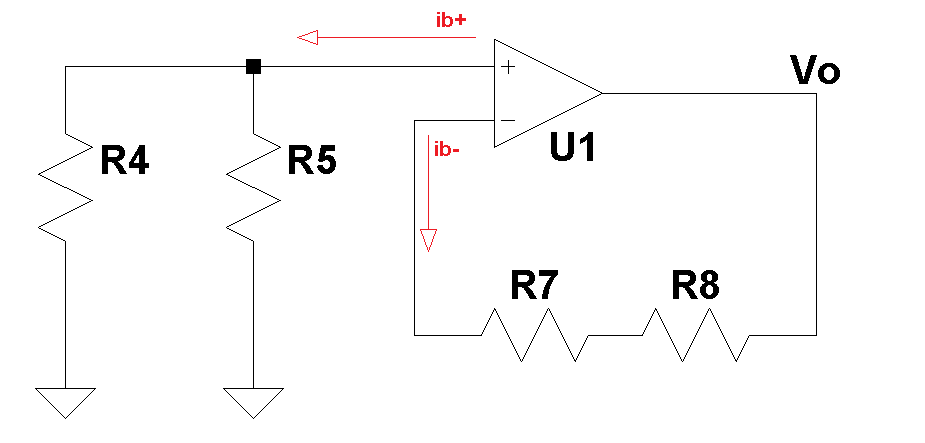
\includegraphics[scale=0.35]{../EJ5/Recursos/circuito_bias.PNG}
    \caption{Etapa amplificaci\'on con el efecto de corrientes de bias}
    \label{fig:pedal_bias}
\end{figure}

\begin{align*}
    & V^{+} = (R_4 // R_5) \cdot ib^{+} \\
    & \frac{V^{-} - V_o}{R_7 + R_8} = ib^{-}
\end{align*}

\begin{equation}
    \Rightarrow V_o = V_{io} + \frac{ib^{+} \cdot R_4}{2} - ib^{-} \cdot (R_7 + R_8)
\end{equation}

Esto demuestra que, el pero caso posible es cuando el potenciometro se encuentra en su m\'aximo punto, en cuyo caso la componente de continua
ser\'a mayor. No obstante, salvo que el amplificador operacional tenga corrientes de bias muy grandes, no deber\'ia tener un efecto muy apreciable.

\begin{table}[H]
    \centering
    \begin{tabular}{c c c c c c}
       Modelo & $GBP$ & $SR$ & $Z_{in}$ & $V_{io}$ & $I_{b}$ \\
       \hline \\
       TL082 & $4MHz$ & $4 \frac{V}{\mu s}$ & $10^{12} \Omega$ & $20mV$ & $8nA$ \\
       LM833 & $15MHz$ & $7 \frac{V}{\mu s}$ & $175k \Omega$ & $5mV$ & $1\mu A$ \\
       LM358 & $1MHz$ & $0,5 \frac{V}{\mu s}$ & No informa & $5mV$ & $150nA$ \\
       \hline
    \end{tabular}
\end{table}

Finalmente, tras haber comparado estos 3 modelos de amplificadores operacionales que se ten\'ian en disponibilidad y con los cuales se estuvieron trabajando previamente,
se opt\'o por trabajar con el TL082 porque es aquel que cumple con todos los requisitos anteriormente mencionados.

\paragraph*{Etapa Alinealidad:} el objetivo de esta etapa es recortar o limitar el rango de tensiones de la se\~nal introduciendo un efecto alineal en la variaci\'on de tensi\'on,
esto implica que la transferencia presenta un efecto no lineal introducido por alg\'un componente, particularmente para ello se emplean diodos. En la figura \ref{fig:circuito_alinealidad} se puede observar
que en principio hay un capacitor $C_5$ cuya funci\'on es la de bloquear el paso de la corriente continua, dejando \'unicamente la alterna sin ning\'un nivel de continua a la salida. Por otro lado, los diodos
est\'an para introducir un efecto alineal en la funci\'on transferencia limitando la senoidal de salida, y la resistencia $R_9$ est\'a colocada de forma tal que limita la corriente y tensi\'on del diodo
cuando se encuentra en funcionamiento para evitar que se quemen, as\'i como tambi\'en establece el valor de la constante de tiempo con la cual la componente de continua deja de ser visible en la salida.

Teniendo en cuenta lo antes dicho, si se analiza el circuito temporalmente primero para la componente de continua, se puede observar que se polariza uno de los diodos que idealmente ser\'a un cable con una ca\'ida de potencial
que puede aproximarse a $VD_{ON} \approx 0,7V$, donde luego circular\'a corriente hasta que el capacitor se termine de carga y para la continua se comporte como circuito abierto. Este \'ultimo estado se alcanza luego que pase cierto tiempo
controlado por la constante de tiempo del sistema que se define como $\tau = R_9 \cdot C_5$. Desde el enfoque de corriente alterna, considerando que el capacitor y la resistencia son vistos como una impedancia, luego la salida de esta 
etapa ser\'a la misma que la entrada siempre y cuando la magnitud se encuentre por debajo de la polarizaci\'on de los diodos, y a partir de dicho punto la salida se ver\'a recortada o saturada en $VD_{ON}$.

Para los diodos de corte se elijen los $1N4148$ porque son diodos rectificadores r\'apidos, entonces pueden responder de mejor manera a las variaciones que se produzcan a la salida del amplificador operacional por el efecto de 
se\~nales de audio que sean complejas, lo cual no podr\'ia pasar quiz\'a con un diodo rectificador com\'un y agregar\'ia distorsiones o efectos no deseados ni intencionados en la salida. Para este diodo la corriente m\'axima de circulaci\'on
en polarizaci\'on directa es de $I_{max} = 300mA$. Si adem\'as se impone un $\tau = 2ms$ se obtiene que $C_5 = 1\mu F$ y $R_9 = 2.2k\Omega$.

\begin{figure}[H]
    \centering
    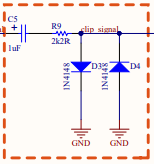
\includegraphics[]{../EJ5/Recursos/circuito_alinealidad.PNG}
    \caption{Circuito de etapa de alinealidad del pedal}
    \label{fig:circuito_alinealidad}
\end{figure}

\paragraph*{Etapa Filtro:} en esta etapa en principio debe asumirse que la resistencia variable $R_{12}$ que est\'a en paralelo al capacitor tiene una impedancia que no quita mucha corriente a la malla del circuito RC, de esta forma se desprecian sus efectos y se considera como si no
estuviera conectado al capacitor, pues de esta forma se simplifica  el an\'alisis. Desde el punto de vista temporal, el circuito RC ante cambios en la entrada modifica la carga del capacitor que acompa\~na cualquier pertubaci\'on o cambio en tal entrada, de esta forma toda
variaci\'on brusca o abrupta que se produzca se ver\'a suavizada por esta etapa, como por ejemplo sucede con el corte de los diodos en la tensi\'on de polarizaci\'on. Desde el punto de vista en frecuencias, este filtro pasabajos limita las frecuencias altas eliminando tales arm\'onicos
que aparezcan por las alinealidades introducidas por la etapa anterior. Por esto \'ultimo, se resuelve la funci\'on transferencia de esta etapa:

\begin{equation}
    H(s) = \frac{1}{1 + s \cdot C_6 \cdot (R_{10} + R_{11})}
\end{equation}

Entonces, considerando que $R_{11}$ es una resistencia variable, se define una frecuencia m\'axima y una m\'inima para establecer el filtro. Considerando $f_{min} = 150Hz$ y $f_{max} = 15kHz$, donde la elecci\'on de estos valores se realiza asumiendo que verdaderamente el sonido audible de una guitarra
no llega a frecuencias superiores a $15kHz$, luego se quiere poder no atenuar ninguna componente o atenuar la mayor parte de ellas como extremos del filtro, para tener un amplio rango de funcionamiento. Finalmente se obtiene que $C_6 = 10nF$, $R_{10} = 1k \Omega$ y $R_{11} = 100k \Omega$. Vale aclarar, que en an\'alisis
de esta etapa no se consider\'o la conexi\'on con la etapa previa puesto que al igual que se viene haciendo con todas las etapas, se impusieron condiciones para independizarlas, principalmente por el hecho de que el filtro busca de cierta forma suavizar los cambios bruscos de la alinealidad y dicha funci\'on se requiere cuando
se logran polarizar los diodos, en cuyo caso la salida de la etapa previa est\'a gobernada por la ca\'ida en los diodos.

\begin{figure}[H]
    \centering
    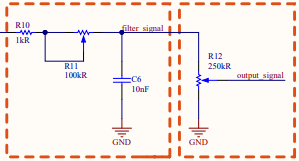
\includegraphics[]{../EJ5/Recursos/circuito_salida.PNG}
    \caption{Circuito etapa de salida o filtro}
    \label{fig:circuito_filtro}
\end{figure}

\paragraph*{Caracterizaci\'on final del sistema:} finalmente se busca utilizar el an\'alisis ya desarrollado para cada etapa de forma independiente, y seg\'un los criterios empleados, llegar a una funci\'on transferencia que describa el funcionamiento
del sistema en su conjunto, analizando desde un punto de vista te\'orico su comportamiento y rangos de operaci\'on. Para esto \'ultimo, como se consideraron criterios que permitieran ver a cada etapa de forma tal que no se cargaran unas a otras, luego la funci\'on transferencia
podr\'ia componerse del producto de las funciones transferencia de cada etapa por separado. No obstante, si se incluye el efecto de la saturaci\'on por el recorte de los diodos, no es posible modelizar correctamente la $H(s)$. Por esto \'ultimo, se plantea la transferencia del sistema
sin la presencia de los diodos y luego se añade tal efecto desde un enfoque cualitativo.

Es necesario hacer una modificaci\'on a las simplificaciones te\'oricas que anteriormente se realizaron, puesto que sin la presencia de los diodos se interconectan las etapas de alinealidad y de filtro de la siguiente manera:

\begin{figure}[H]
    \centering
    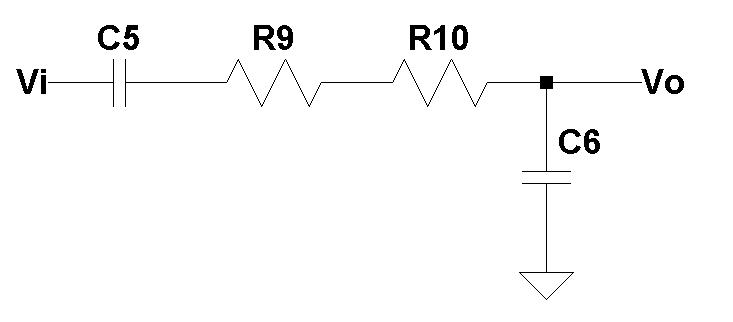
\includegraphics[scale=0.4]{../EJ5/Recursos/circuito_correccion.PNG}
    \caption{Circuito corregido de etapas sin diodos}
    \label{fig:circuito_sin_diodos_pedal}
\end{figure}

Donde para obtener la funci\'on transferencia que caracteriza a esta etapa del sistema basta con realizar un divisor de tensi\'on y luego operar algebraicamente
para llegar a la expresi\'on siguiente.

\begin{align*}
    H_{etapa}(s) &= \frac{V_o}{V_i} = \frac{\frac{1}{s \cdot C_6}}{\frac{1}{s \cdot C_5} + \frac{1}{s \cdot C_6} + R_9 + R_10} \\
    & 
    \Rightarrow C_p = C_5 // C_6 = \frac{C_5 \cdot C_6}{C_5 + C_6}
    \Rightarrow
    H_{etapa}(s) = \frac{C_5}{C_5 + C_6} \cdot \frac{1}{1 + s \cdot C_p \cdot (R_1 + R_2)}
\end{align*}

Por lo tanto, ahora s\'i si obtiene la transferencia total del sistema como el conjunto de las etapas.

\begin{equation*}
    H(s) = \frac{s \cdot R_p \cdot C_2}{1 + s \cdot C_2 \cdot R_p} \cdot \frac{1 + s \cdot (1 + \frac{R_7}{R_6}) \cdot C_3 \cdot R_6}{1 + s \cdot C_3 \cdot R_6} \cdot \frac{C_5}{C_5 + C_6} \cdot \frac{1}{1 + s \cdot C_p \cdot (R_1 + R_2)}
\end{equation*}

\begin{equation}
    H(s) = \frac{\frac{s}{2\pi \cdot 2.05Hz}}{1 + \frac{s}{2 \pi \cdot 2.05Hz}} \cdot \frac{1 + \frac{s}{2 \pi \cdot 0,79Hz}}{1 + \frac{s}{2\pi \cdot 1,59Hz}} \cdot \frac{0.99}{1 + \frac{s}{2 \pi \cdot 5.02kHz}}
\end{equation}

Vale mencionar que este an\'alisis no tiene en cuenta las posibles variaciones del sistema cuando se regula la distorsi\'on y el tono con los potenciometros agregados, puesto que bajo dichos casos se mueve
la forma de la respuesta en frecuencia de la caracterizaci\'on obtenida, tanto de forma vertical como horizontal. Esto se debe a que la variaci\'on de la distorsi\'on implica modificar la ganancia de la banda pasante,
y controlar el tono implica modificar la frecuencia de corte del filtro pasabajos utilizado en la \'ultima etapa. Esta regulaci\'on de ganancia y frecuencias fueron establecidas con el objetivo de permitir alcanzar un rango de operaci\'on
amplio, ya que al poder elevar mucho la ganancia y modificar la frecuencia de corte, se puede ajustar seg\'un se prefiera la banda pasante, logrando un ancho de banda seg\'un se lo desea con amplitudes que pueden variar dentro de un rango
grande respecto de lo que se esperar\'ia a la salida de un instrumento. Esto \'ultimo se tomo como criterio puesto que se esperaba que el resultado final fuera versatil a la hora de su manejo.

\subsection{Simulaci\'on de etapas}
Se simularon cada una de las etapas por separa para analizar su comportamiento, el cual puede ilustrarse de forma breve a continuaci\'on con las respuestas de dichos sistemas a una exitaci\'on.
Vale aclarar, que la simulaci\'on del conjunto de las etapas es realizada en la subsecci\'on de Resultados donde se contrastan las respuestas en frecuencia de la medici\'on y lo te\'orico, superponiendo
tales curvas con la simulaci\'on en LTSpice habiendo empleado un montecarlo para incluir variaci\'on por tolerancia de componentes.

\begin{figure}[H]
    \centering
    \caption{Simulaci\'on de etapas}
    \begin{tabular}{c c}
        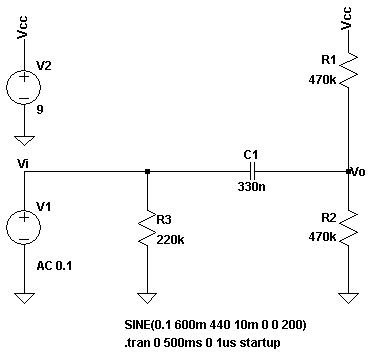
\includegraphics[scale=0.5]{../EJ5/Recursos/Simulaciones/circuito_offset.png} &
        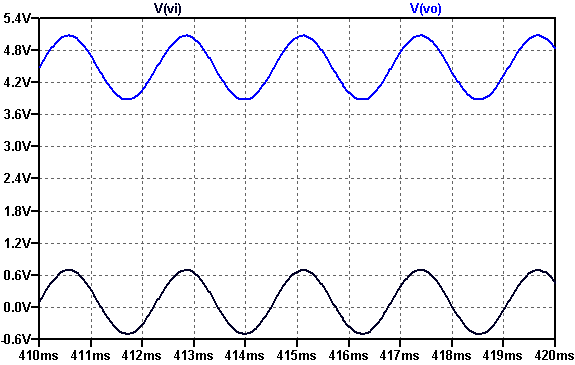
\includegraphics[scale=0.47]{../EJ5/Recursos/Simulaciones/medicion_offset.png} \\
        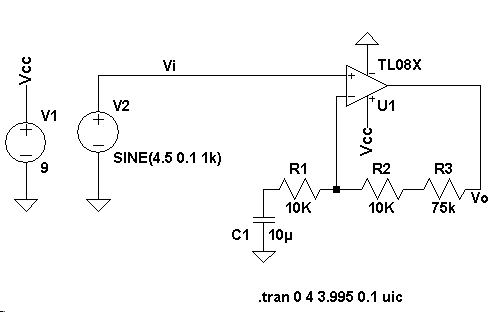
\includegraphics[scale=0.5]{../EJ5/Recursos/Simulaciones/circuito_ampli.png} &
        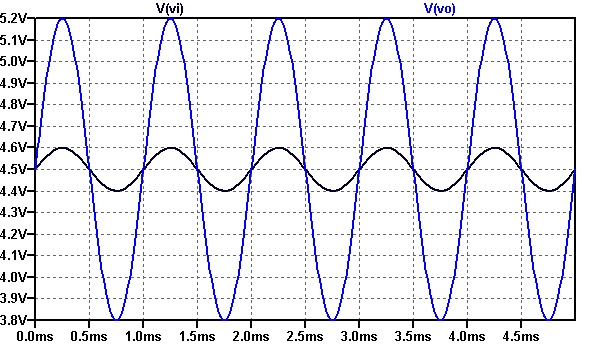
\includegraphics[scale=0.45]{../EJ5/Recursos/Simulaciones/medicion_ampli.png} \\
        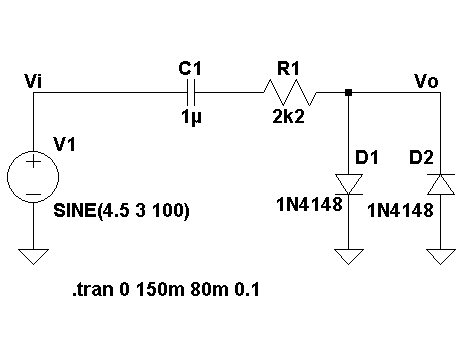
\includegraphics[scale=0.5]{../EJ5/Recursos/Simulaciones/circuito_alineal.png} &
        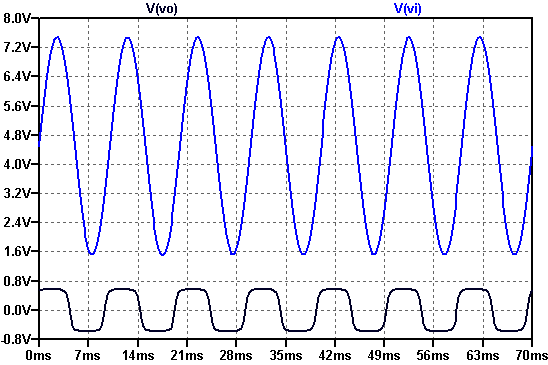
\includegraphics[scale=0.5]{../EJ5/Recursos/Simulaciones/medicion_alineal.png} \\
        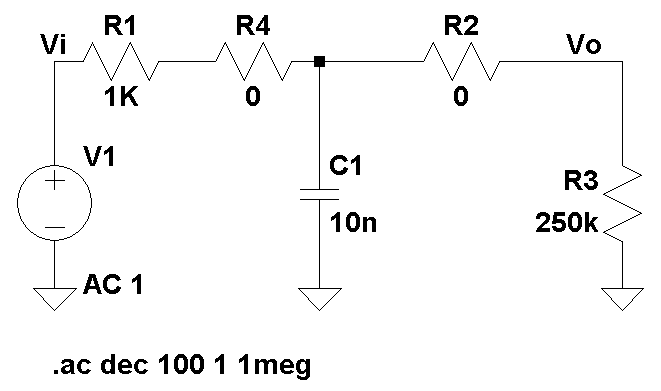
\includegraphics[scale=0.40]{../EJ5/Recursos/Simulaciones/circuito_filtro.png} &
        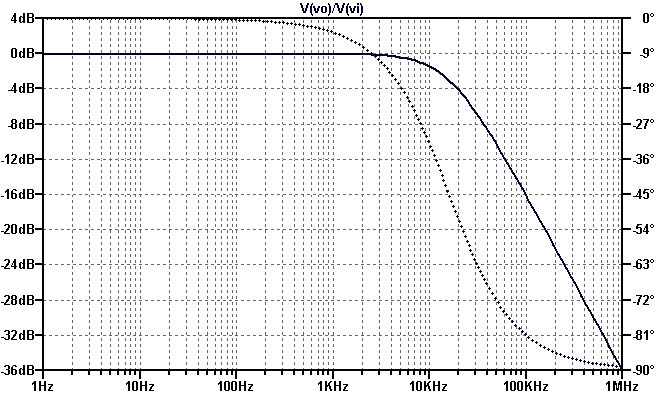
\includegraphics[scale=0.43]{../EJ5/Recursos/Simulaciones/medicion_filtro.png} \\
    \end{tabular}
    \label{fig:simulacion_pedal}
\end{figure}

\subsection{Resultados}

\paragraph*{An\'alisis de rango} se decidi\'o tomar tres frecuencias diferentes para las cuales aplicar una se\~nal senoidal en la entrada del circuito de distorsi\'on y evaluar
los valores de tensi\'on pico a pico a partir de los cuales o bien el circuito era incapaz de saturar, o no hab\'ia forma de evitar que el amplificador operacional se saturar\'a, para de este forma,
tener una noci\'on representativa del rango de funcionamiento del dispositivo armado.

\begin{table}[H]
    \centering
    \begin{tabular}{c c c}
        $f [Hz]$ & $V_{pp}$ donde no satura nunca & $V_{pp}$  donde satura siempre \\
        \hline \\
        $20$ & $10mV$ & $1.5V$ \\
        $440$ & $20mV$ & $1.4V$ \\
        $3600$ & $25mV$ & $1.3V$ \\ 
        \hline \\
    \end{tabular}
    \caption{Mediciones para rango de operaci\'on}
\end{table}

\paragraph*{Respuesta en frecuencia:} se mide la respuesta en frecuencia del circuito sin considerar los diodos, es decir, desconectandolos del mismo, puesto que el circuito
dejar\'ia de considerarse lineal y por ello no tendr\'ia sentido analizar tal respuesta en frecuencia. Desde este enfoque, se observan el bode resultante de la medici\'on, la simulaci\'on 
y los c\'alculos te\'oricos, para esto \'ultimo se consideraron las aproximaciones tomadas donde las etapas eran independientes unas de otras, es decir que no se cargaban entre s\'i y se multiplicaron
para obtener una funci\'on transferencia resultante.

\begin{figure}[H]
    \centering
    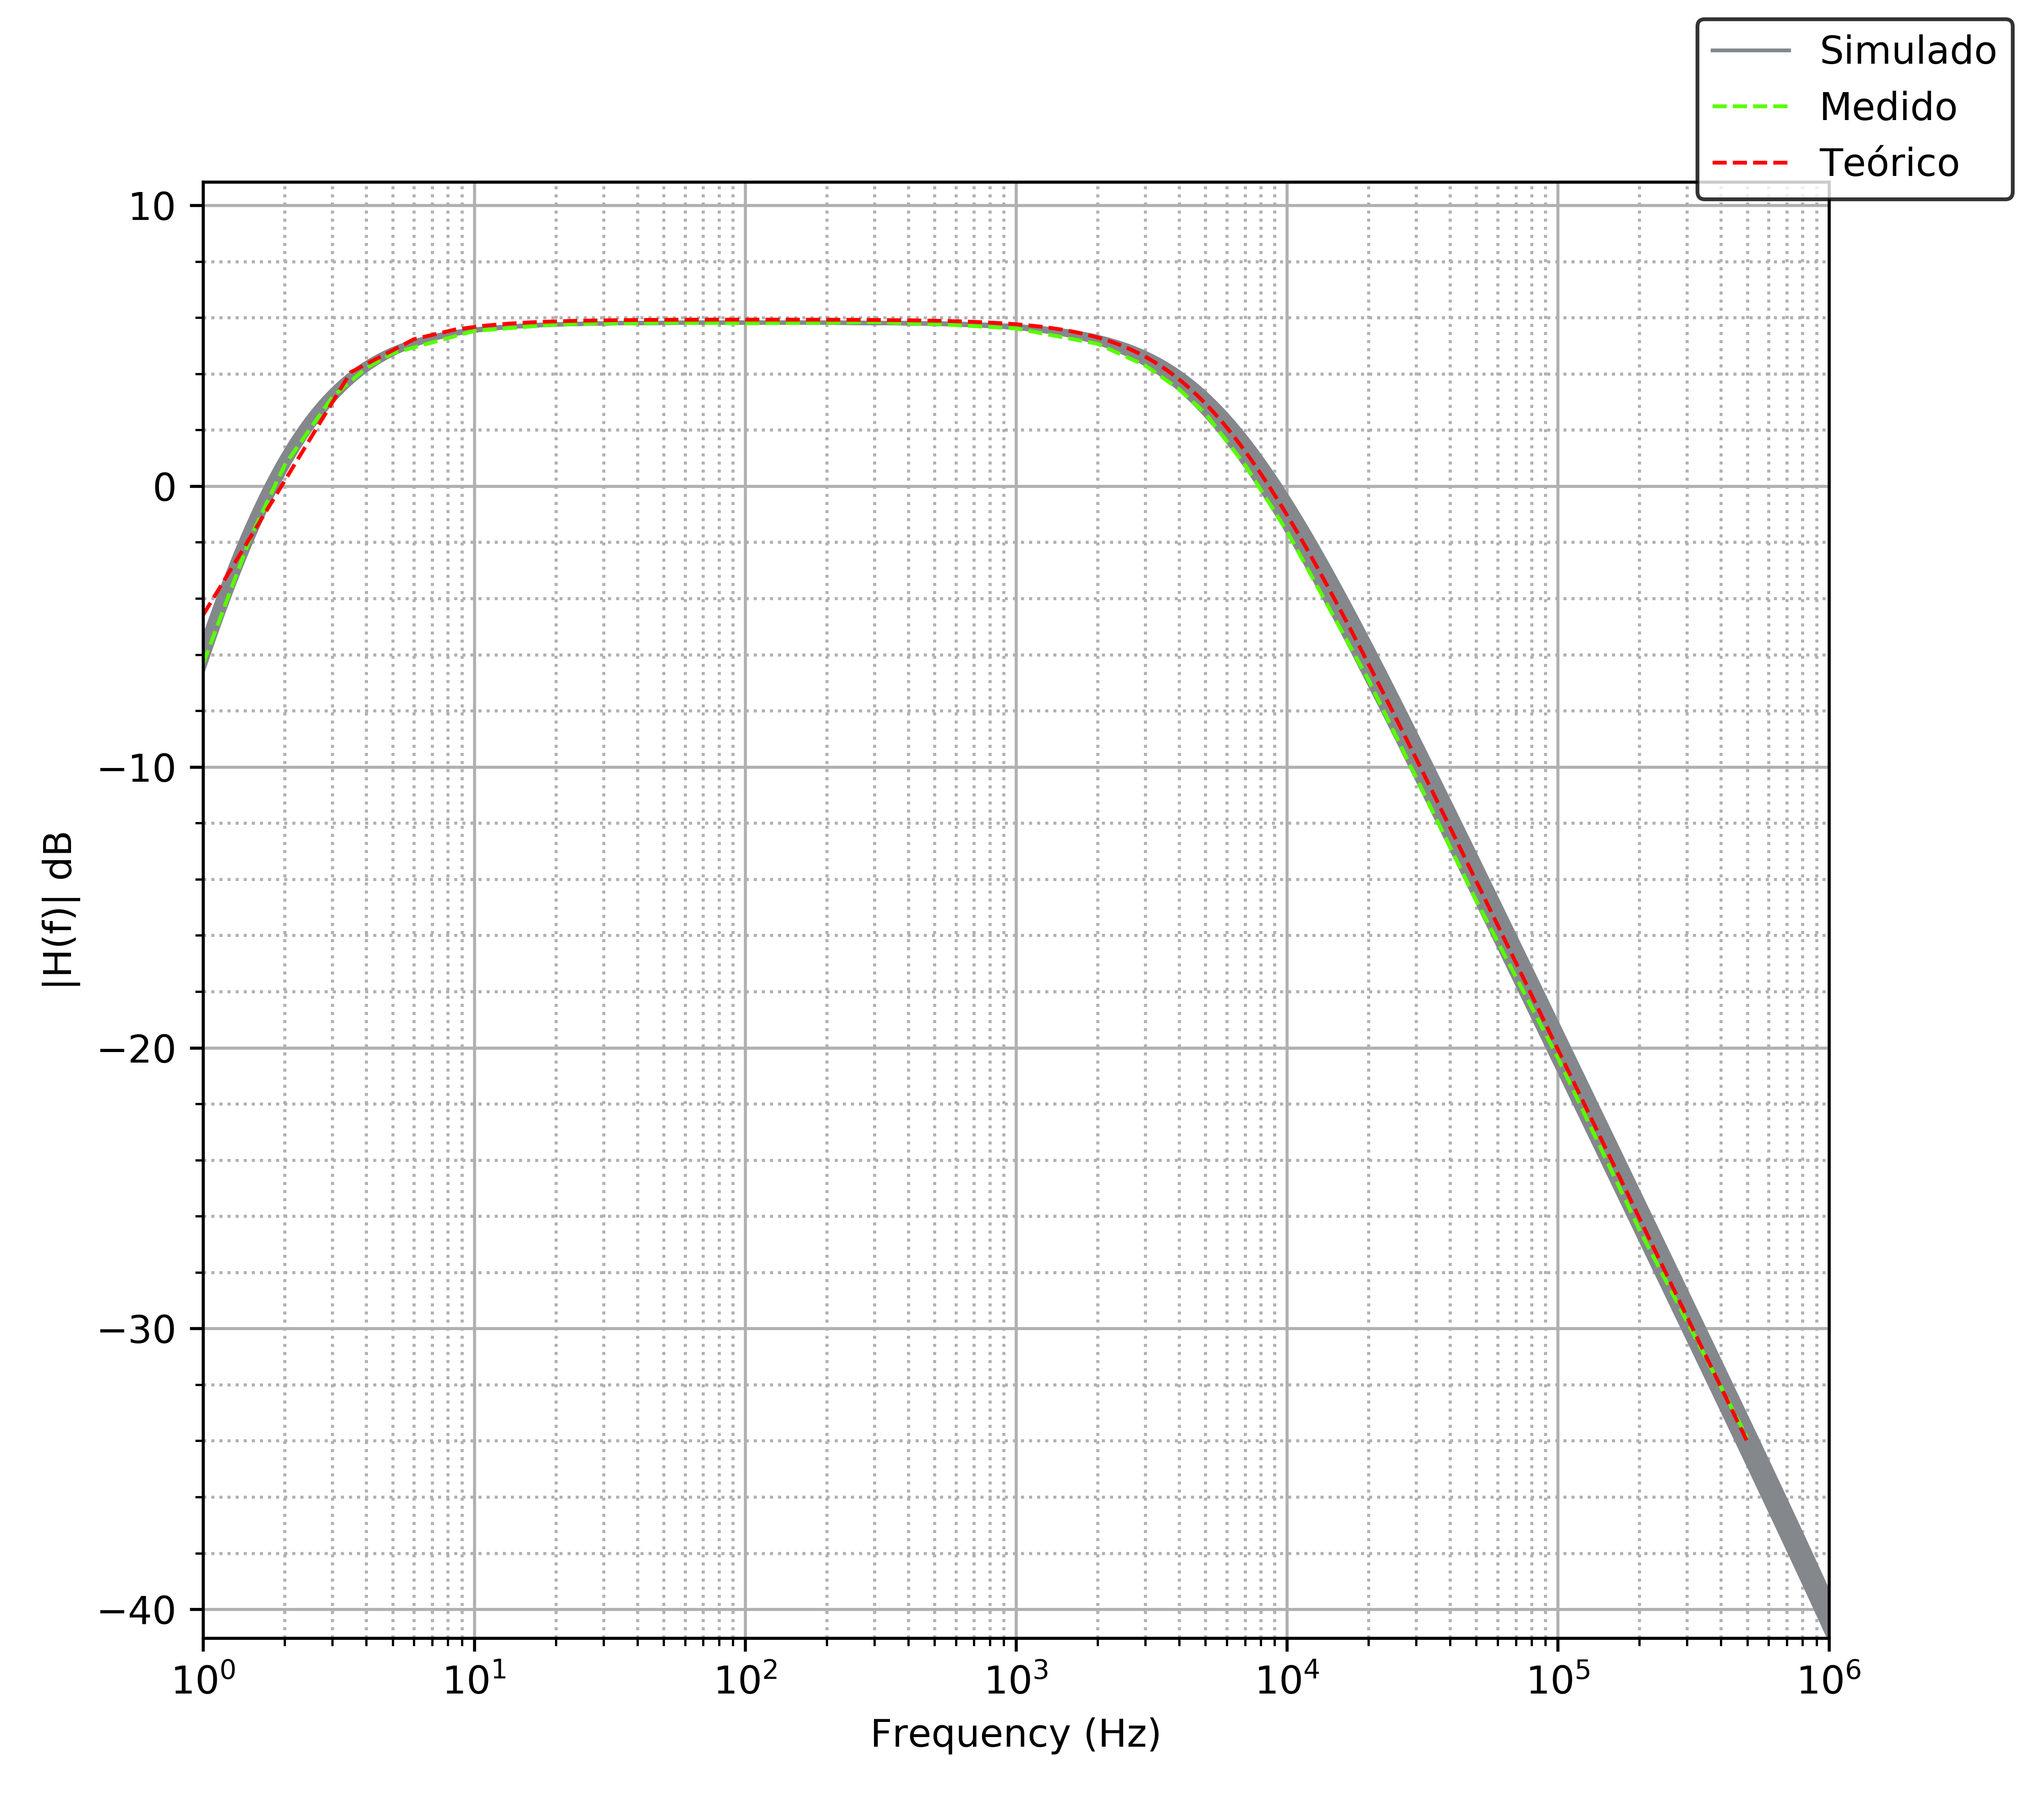
\includegraphics[scale=0.6]{../EJ5/Recursos/bode_modulo.png}
    \caption{Diagrama de bode en m\'odulo del pedal}
    \label{fig:pedal_bode_modulo}
\end{figure}

\begin{figure}[H]
    \centering
    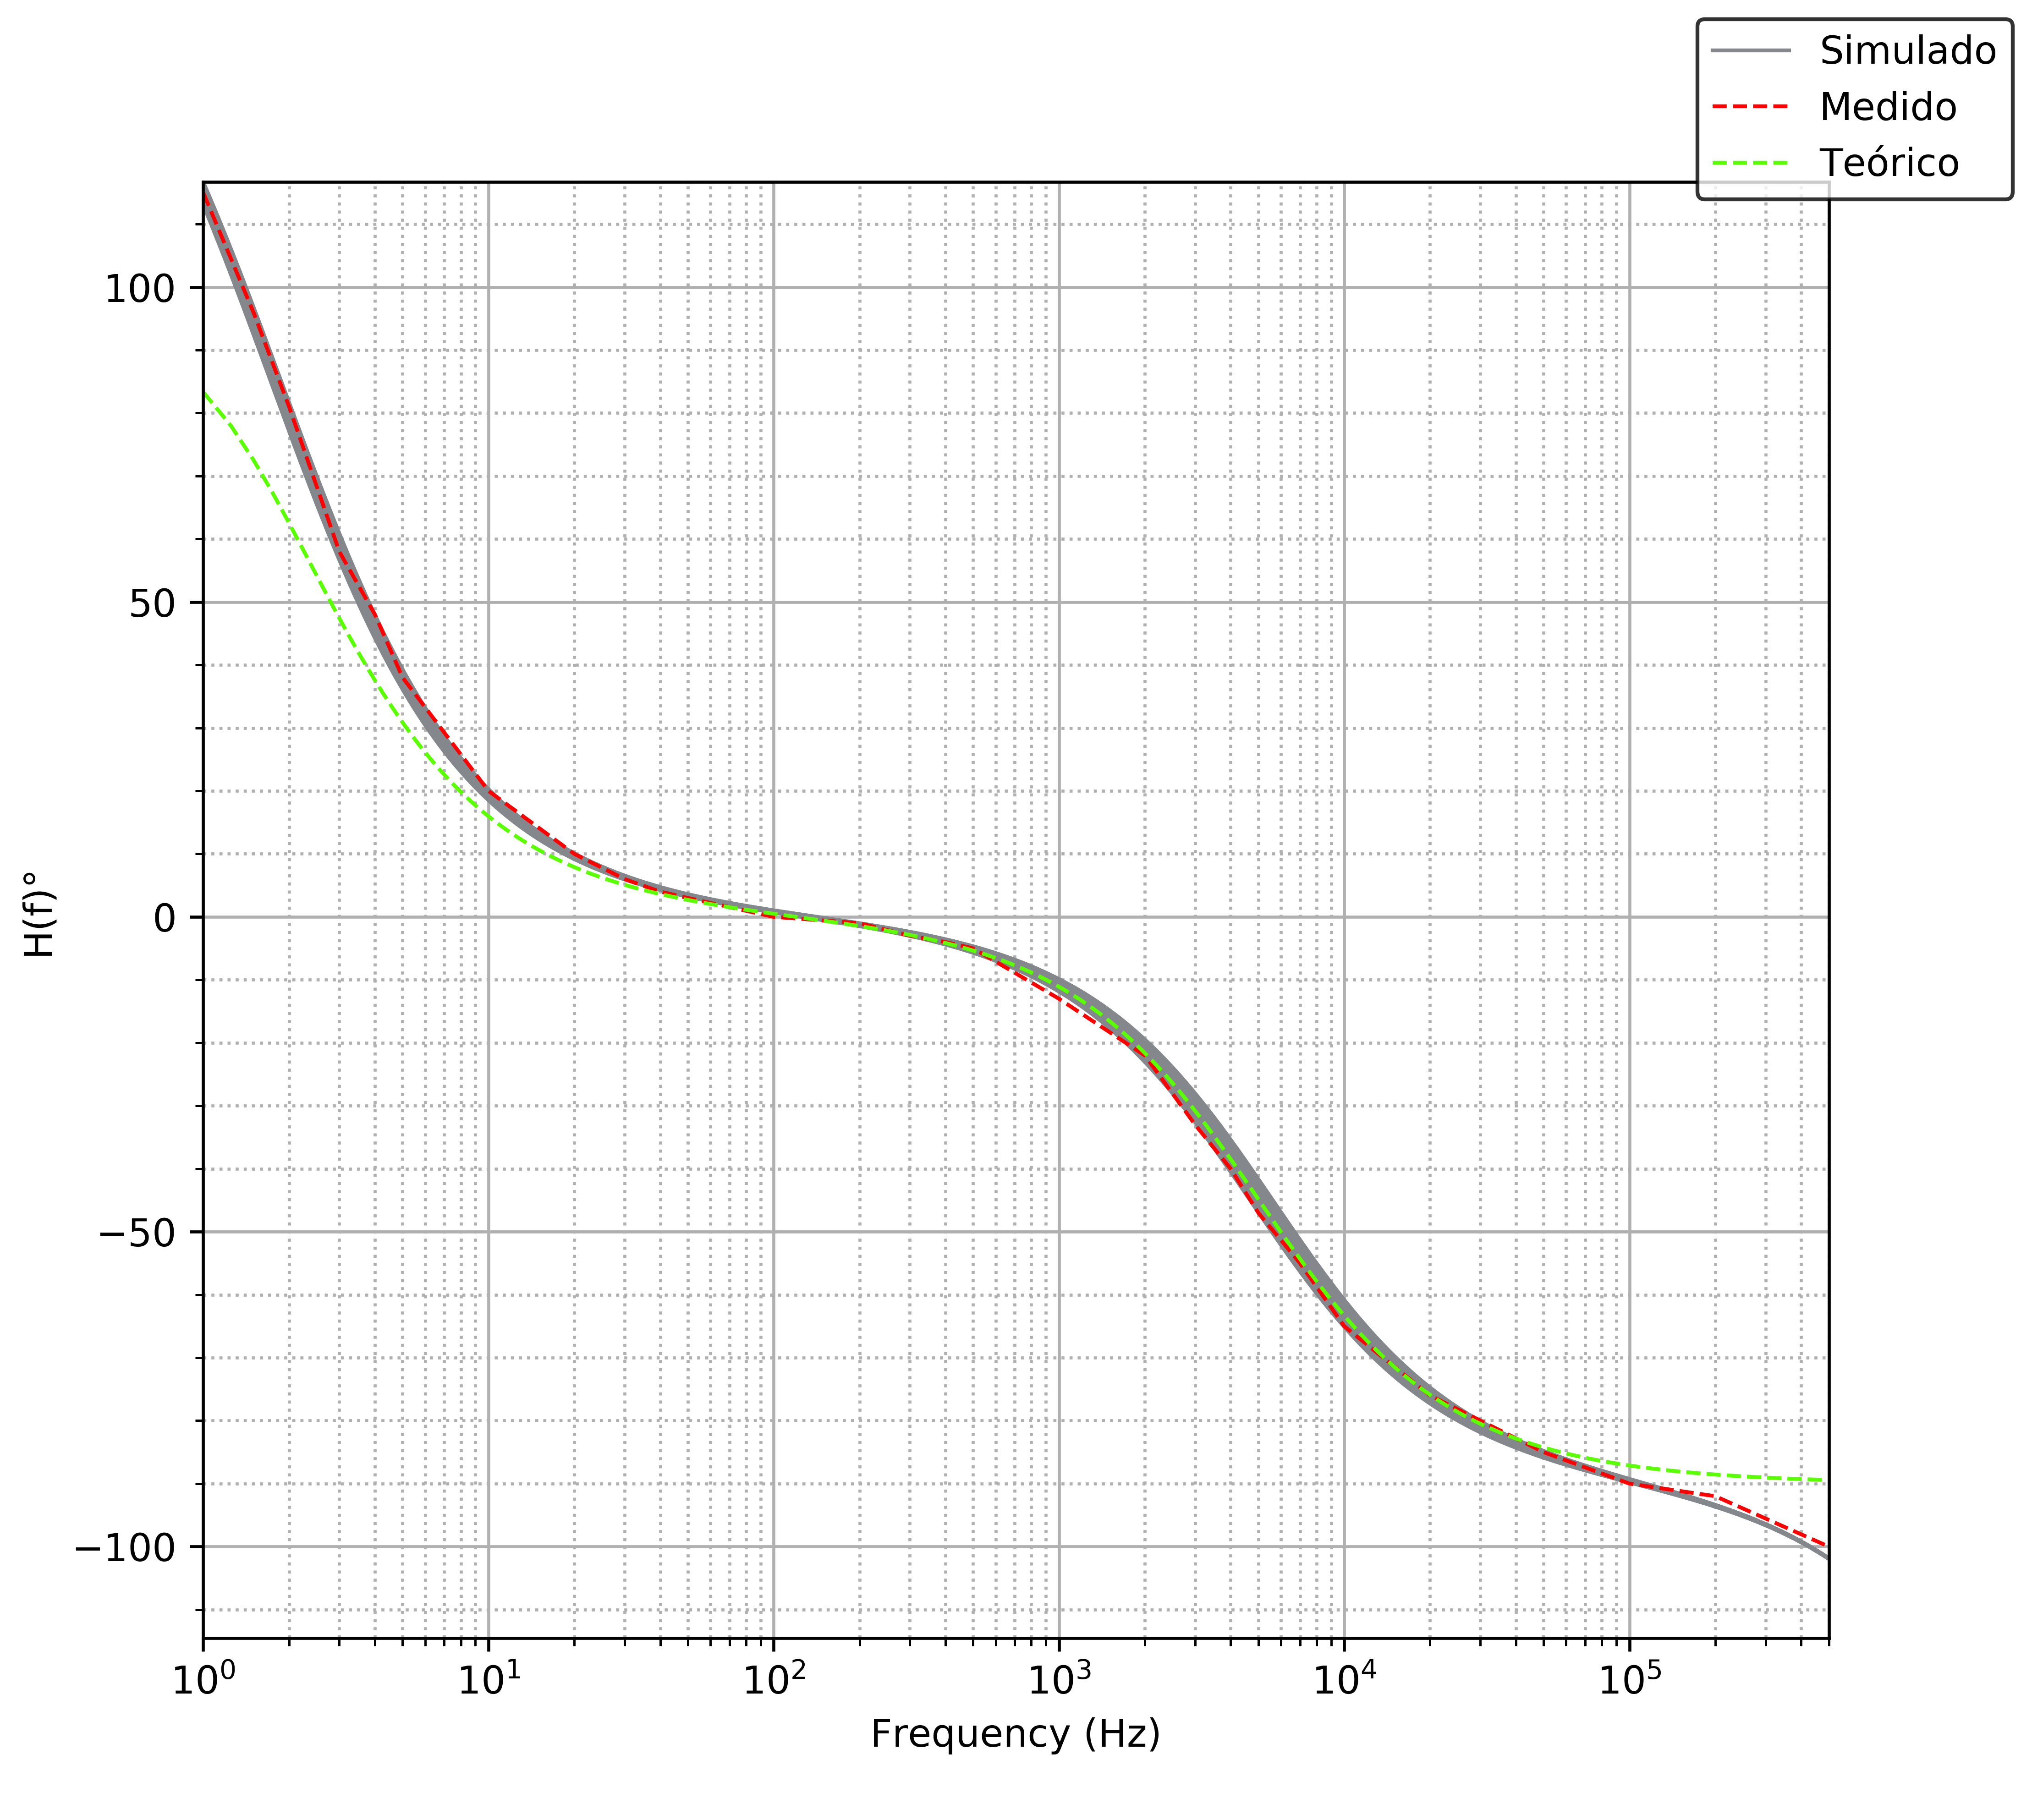
\includegraphics[scale=0.6]{../EJ5/Recursos/bode_fase.png}
    \caption{Diagrama de bode en fase del pedal}
    \label{fig:pedal_bode_fase}
\end{figure}

Es importante aclarar que para tales mediciones, simulaciones y c\'alculos, se consideran los potenciometros que controlan la distorsi\'on y el control de tonos al m\'inimo, pues de esta forma los efectos
est\'an minimizado, ergo, es por ello que se produce que en la respuesta en frecuencia obtenida se aten\'uan frecuencia que est\'an dentro del espectro audible, puesto que si se aumentar\'a la ganancia de la banda pasante luego
se producir\'ia una distorsi\'on sin atenuar el espectro audible, tal y como fue consignado y dise\~nado.

\paragraph*{Respuesta temporal:} se utilizaron dos se\~nales senoidales de frecuencias $f = 440Hz$ y $f = 3600Hz$, configurando dos casos distintos, donde los potenciometros que regulan
la distorsi\'on y el tono se encontraban en su posici\'on m\'inima, y luego donde se encontraban en un punto medio cualquiera donde se produjera una dada distorsi\'on. Ante esto, se realizaron mediciones sobre
cada una de las etapas del circuito para poder establecer los efectos que cada una de ellas produc\'ian sobre la se\~nal. A continuaci\'on se presentan los resultados medidos, t\'engase en cuenta que en las mediciones
los cuatro gr\'aficos contienen una se\~nal amarilla que corresponde a la entrada original y luego una verde correspondiente al resultado de cada etapa, donde el orden de los gr\'aficos de izquierda a derecha y de arriba hacia abajo est\'a dado
como etapa de offset, etapa de amplificaci\'on, etapa de alinealidad y finalmente la etapa del filtro.

\begin{figure}[H]
    \centering
    \begin{tabular}{c c}
        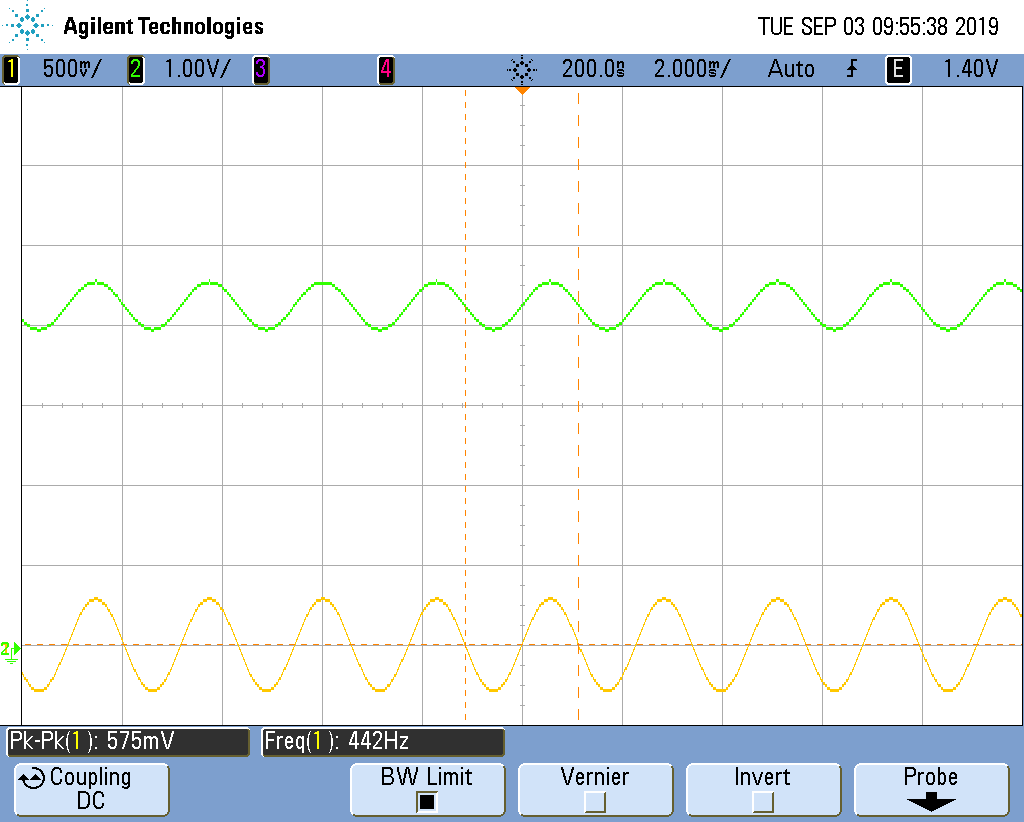
\includegraphics[scale=0.2]{../EJ5/Mediciones/Osciloscopio/Senoide_440_Minimo/scope_1.png} &
        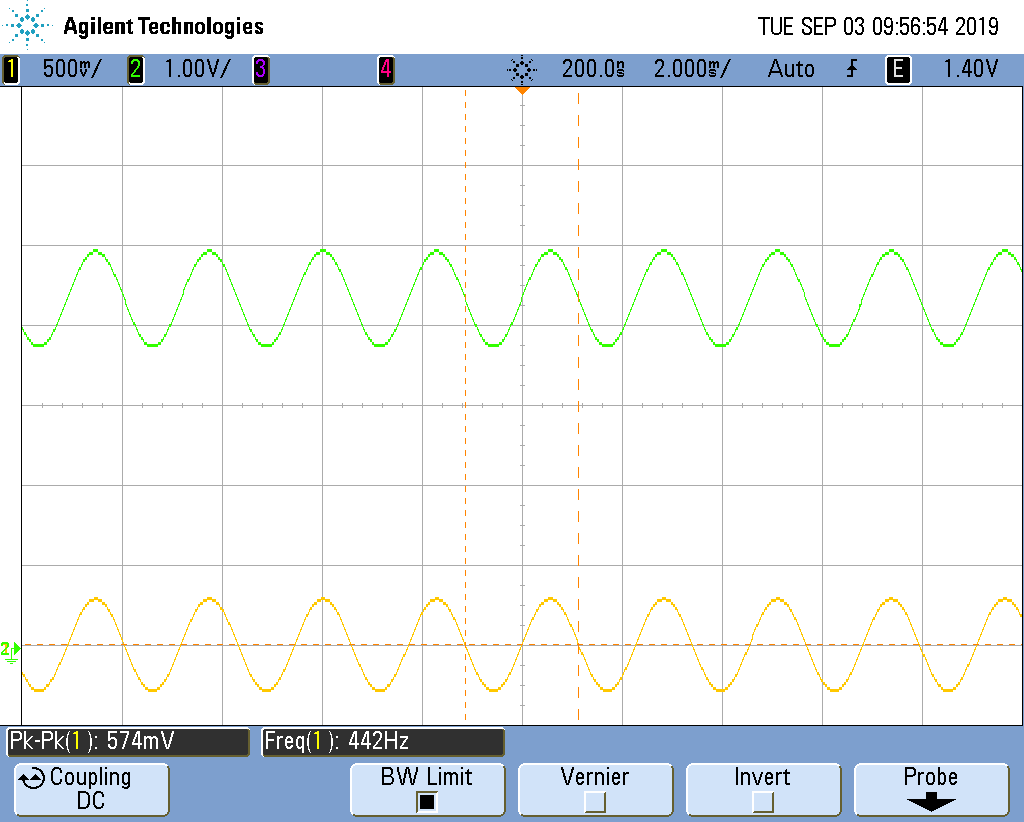
\includegraphics[scale=0.2]{../EJ5/Mediciones/Osciloscopio/Senoide_440_Minimo/scope_2.png} \\
        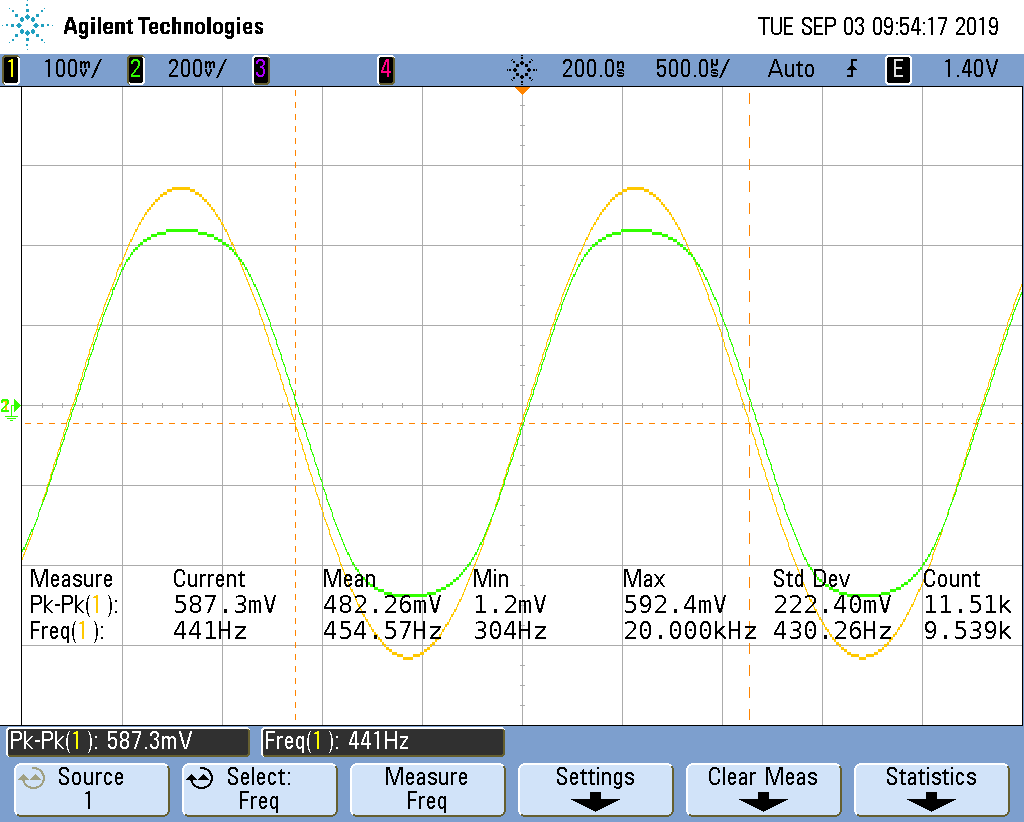
\includegraphics[scale=0.2]{../EJ5/Mediciones/Osciloscopio/Senoide_440_Minimo/scope_0.png} &
        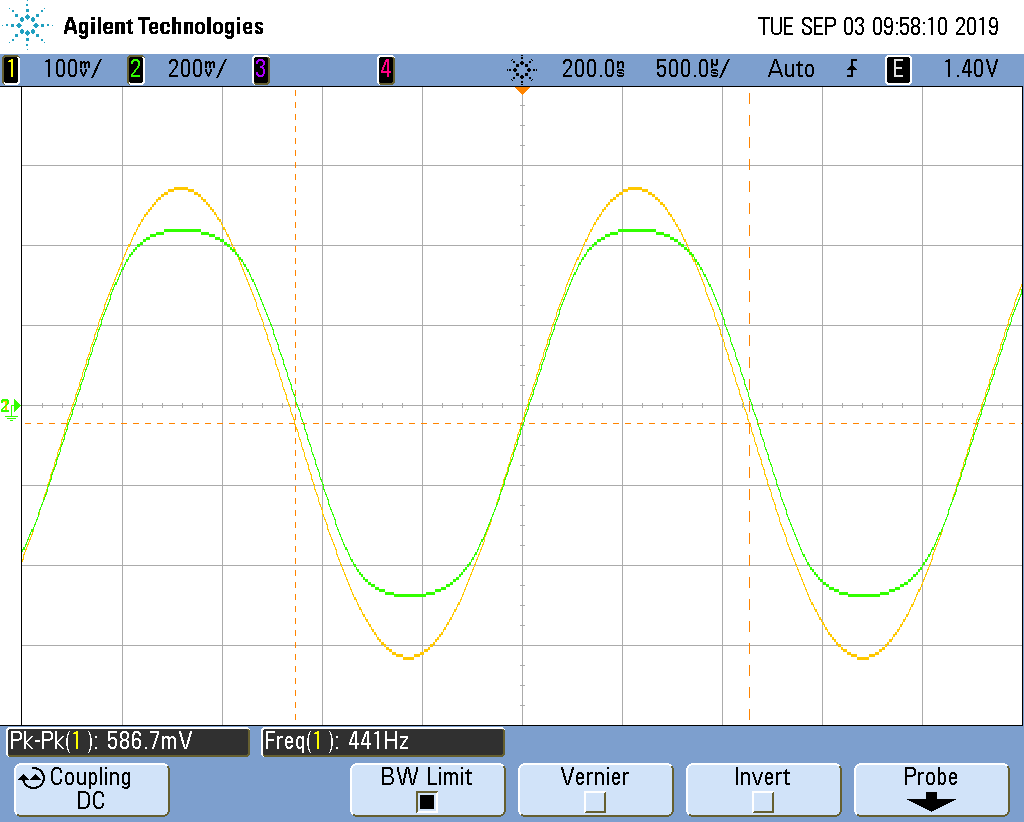
\includegraphics[scale=0.2]{../EJ5/Mediciones/Osciloscopio/Senoide_440_Minimo/scope_3.png} 
    \end{tabular}
    \caption{Casos para senoidal de 440Hz con potenciometros al m\'inimo}
    \label{fig:senoide_440_minimo}
\end{figure}

\begin{figure}[H]
    \centering
    \begin{tabular}{c c}
        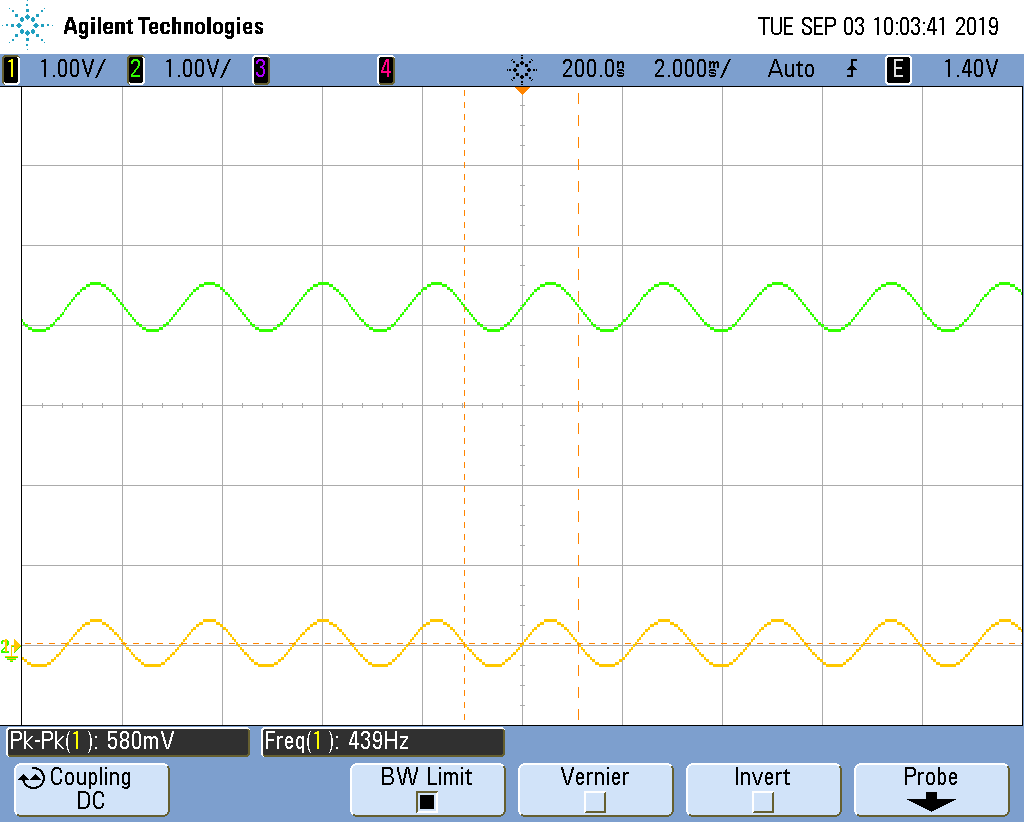
\includegraphics[scale=0.2]{../EJ5/Mediciones/Osciloscopio/Senoide_440_Medio/scope_5.png} &
        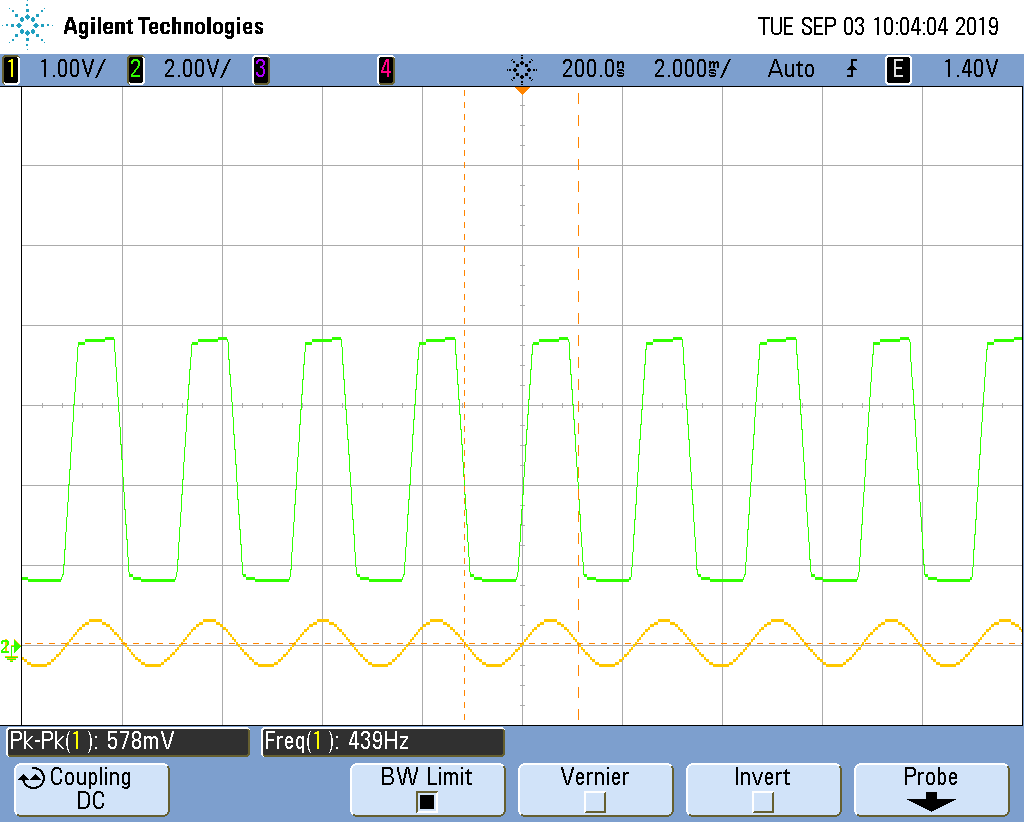
\includegraphics[scale=0.2]{../EJ5/Mediciones/Osciloscopio/Senoide_440_Medio/scope_6.png} \\
        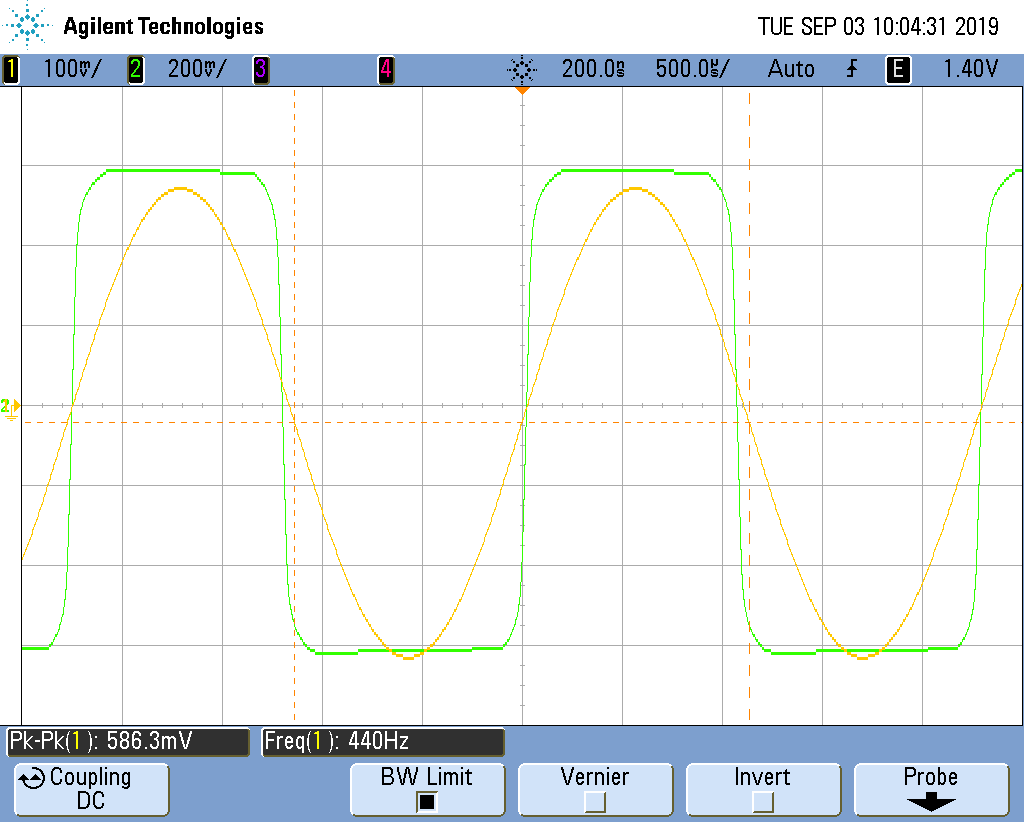
\includegraphics[scale=0.2]{../EJ5/Mediciones/Osciloscopio/Senoide_440_Medio/scope_7.png} &
        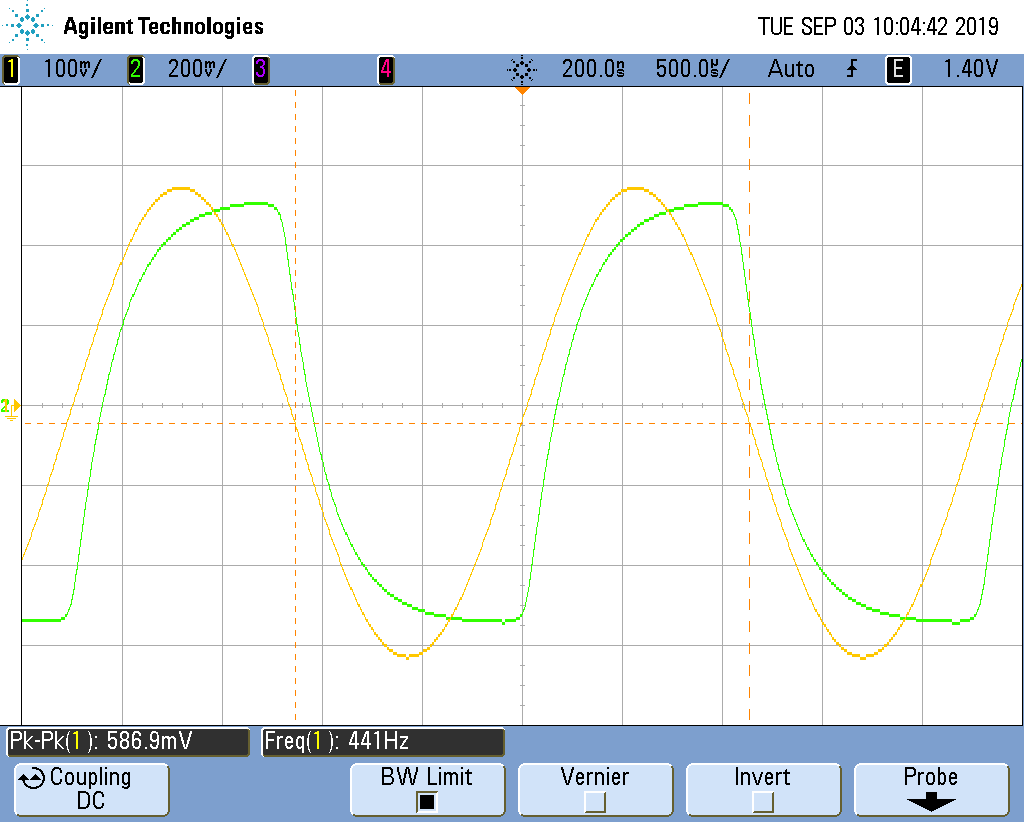
\includegraphics[scale=0.2]{../EJ5/Mediciones/Osciloscopio/Senoide_440_Medio/scope_8.png} 
    \end{tabular}
    \caption{Casos para senoidal de 440Hz con potenciometro en alg\'un estado}
    \label{fig:senoide_440_medio}
\end{figure}

\begin{figure}[H]
    \centering
    \begin{tabular}{c c}
        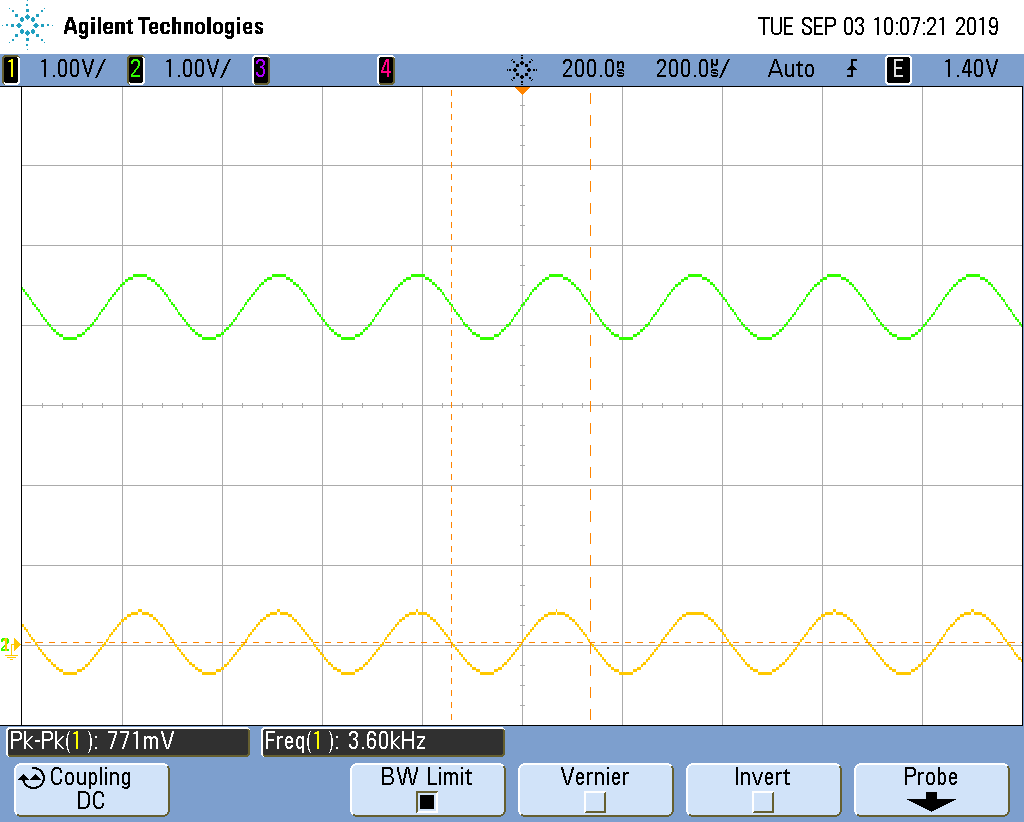
\includegraphics[scale=0.2]{../EJ5/Mediciones/Osciloscopio/Senoide_3600_Minimo/scope_9.png} & 
        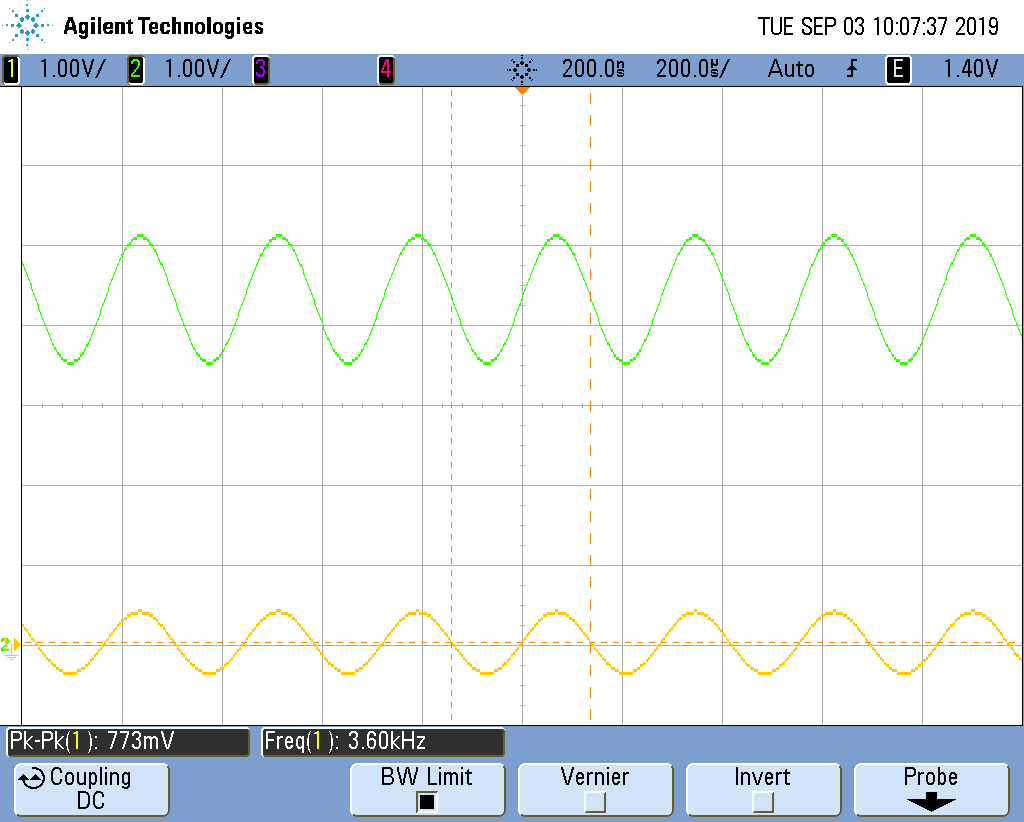
\includegraphics[scale=0.2]{../EJ5/Mediciones/Osciloscopio/Senoide_3600_Minimo/scope_10.png} \\
        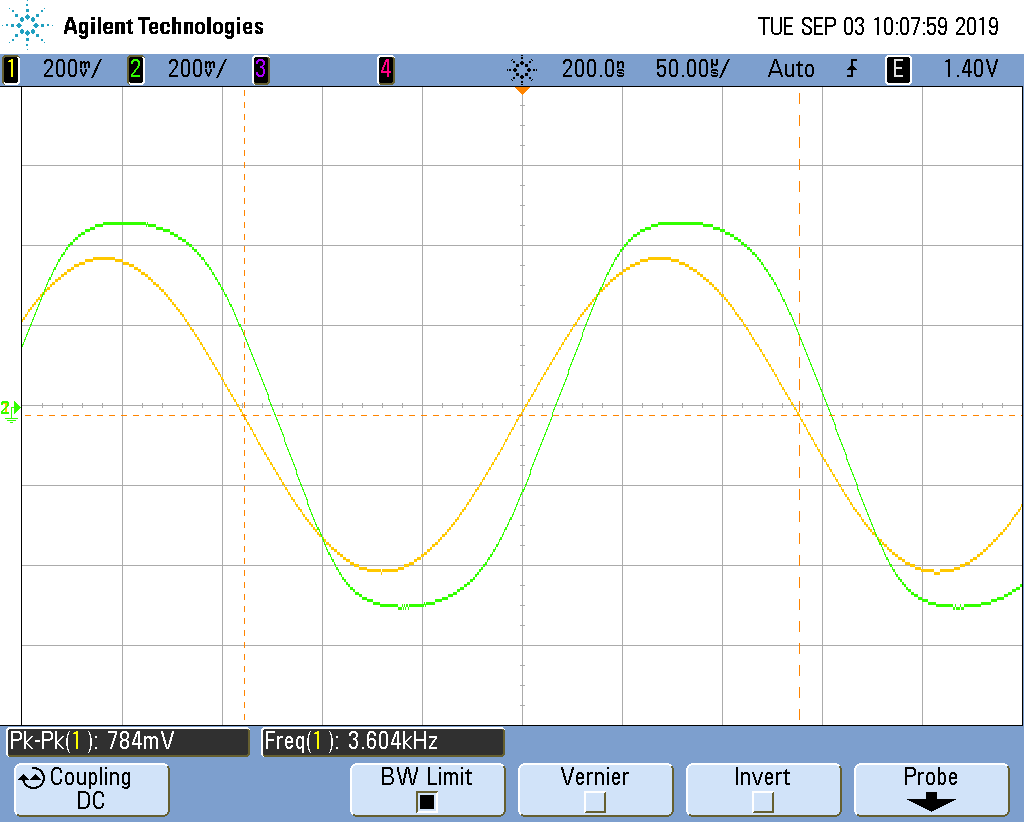
\includegraphics[scale=0.2]{../EJ5/Mediciones/Osciloscopio/Senoide_3600_Minimo/scope_11.png} & 
        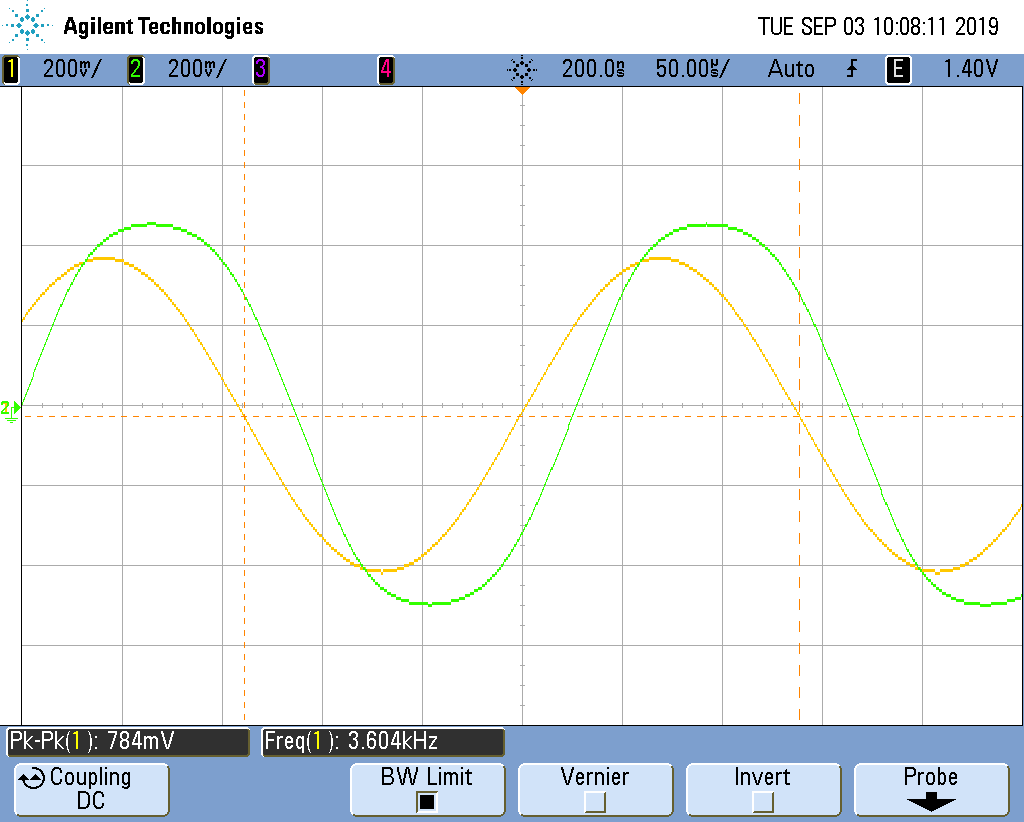
\includegraphics[scale=0.2]{../EJ5/Mediciones/Osciloscopio/Senoide_3600_Minimo/scope_12.png} 
    \end{tabular}
    \caption{Casos para senoidal de 3600Hz con potenciometros al m\'inimo}
    \label{fig:senoide_3600_minimo}
\end{figure}

\begin{figure}[H]
    \centering
    \begin{tabular}{c c}
        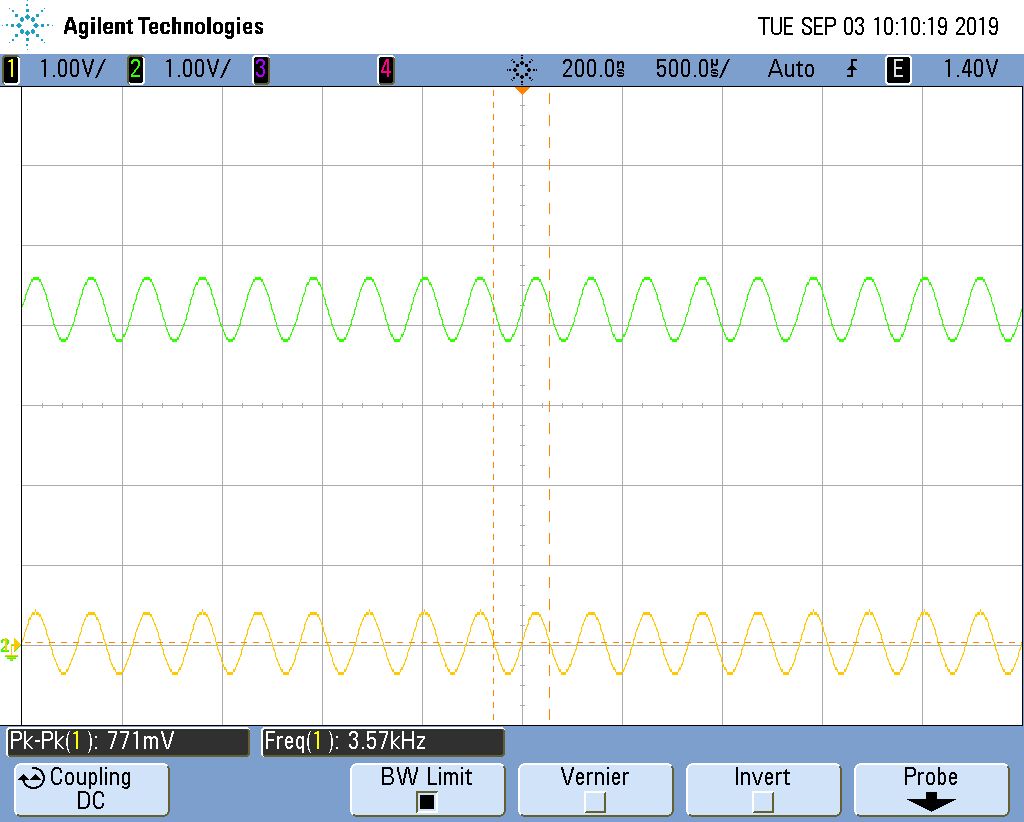
\includegraphics[scale=0.2]{../EJ5/Mediciones/Osciloscopio/Senoide_3600_Medio/scope_13.png} &
        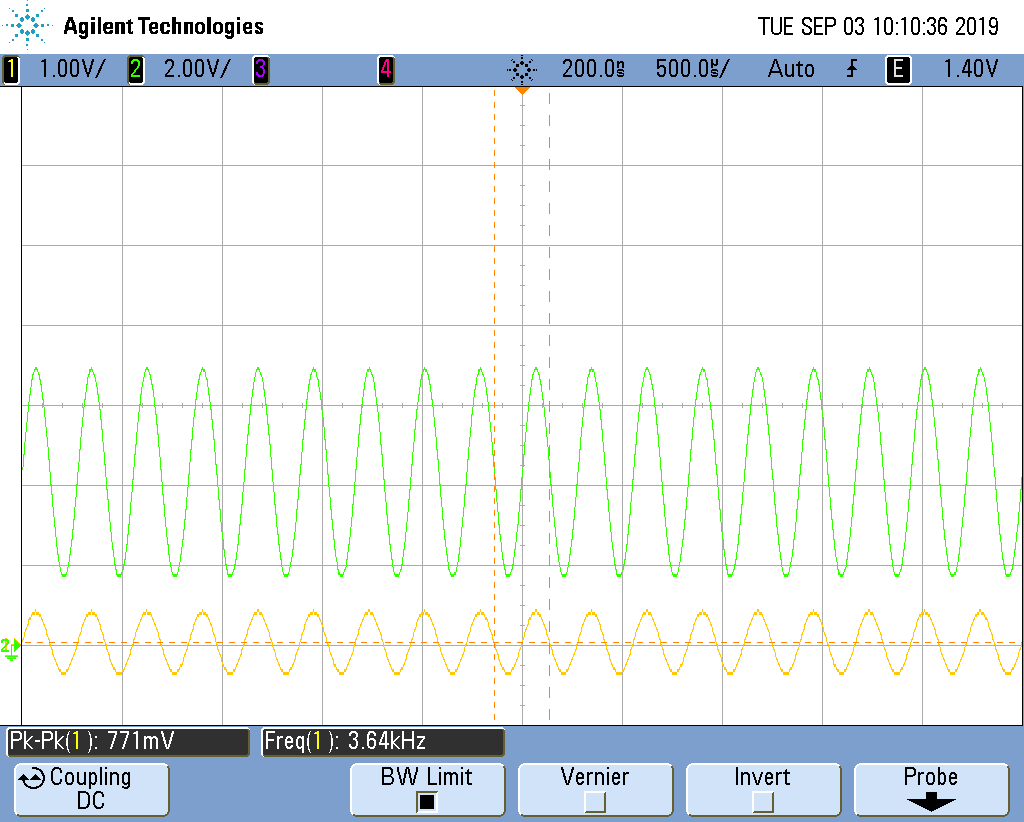
\includegraphics[scale=0.2]{../EJ5/Mediciones/Osciloscopio/Senoide_3600_Medio/scope_14.png} \\
        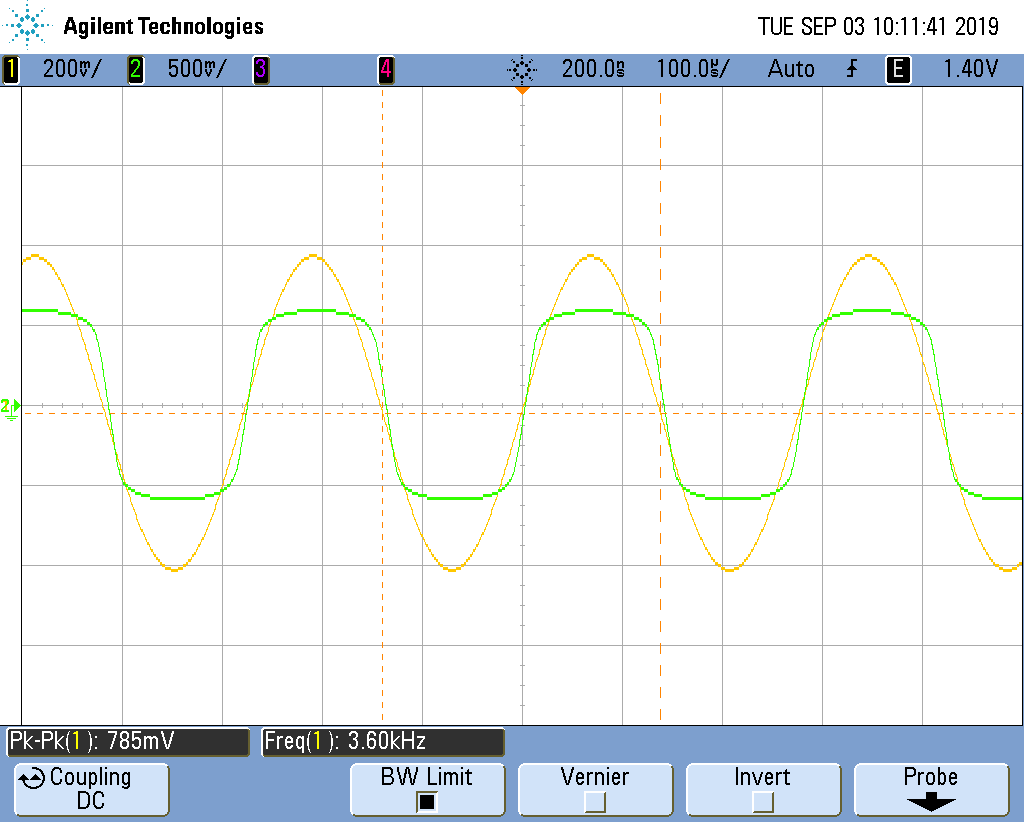
\includegraphics[scale=0.2]{../EJ5/Mediciones/Osciloscopio/Senoide_3600_Medio/scope_16.png} &
        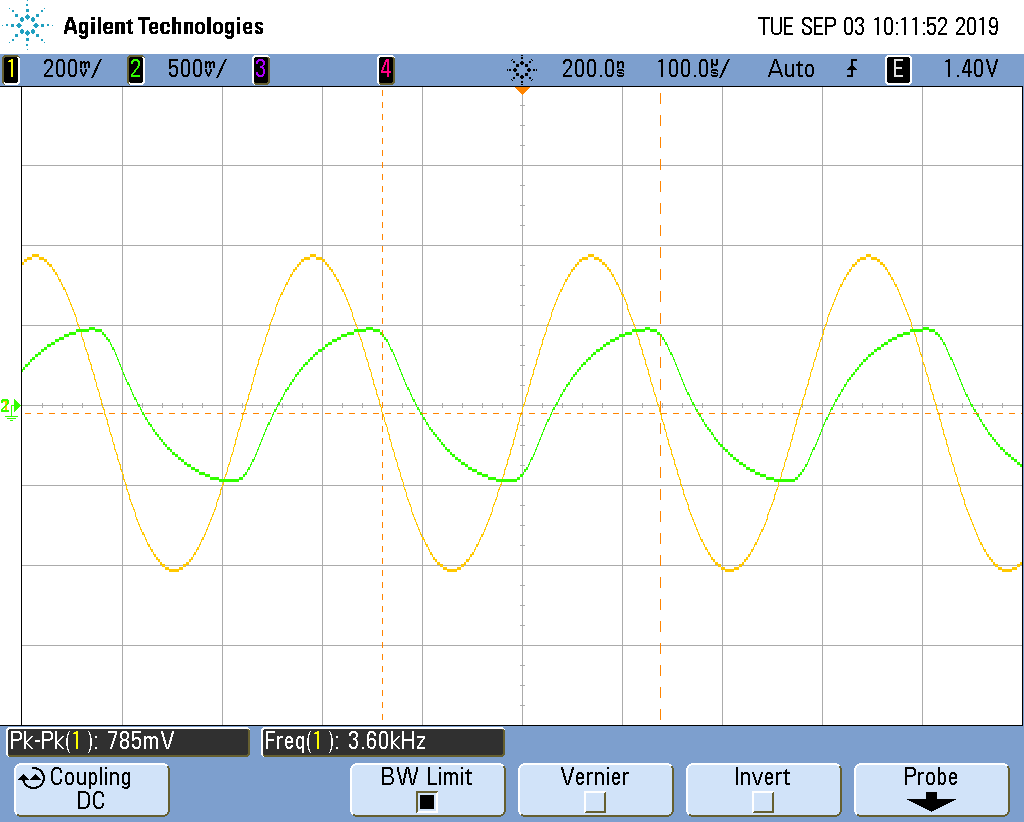
\includegraphics[scale=0.2]{../EJ5/Mediciones/Osciloscopio/Senoide_3600_Medio/scope_17.png}
    \end{tabular}
    \caption{Casos para senoidal de 3600Hz con potenciometros en alg\'un estado}
    \label{fig:senoide_3600_medio}
\end{figure}

\subsection{Implementaci\'on pr\'actica}

\paragraph*{Esquem\'atico:} en el circuito se pueden observar cada una de las etapas ya mencionadas y analizadas en el apartado te\'orico de la presente secci\'on,
pero adem\'as, se incluyen consideraciones pr\'acticas del dise\~no en PCB, como la conexi\'on como buffer del amplificador operacional no utilizado para evitar que entre
en un modo de oscilaci\'on que introduzca efectos no deseados al circuito, capacitor $C_7$ de desacople para el circuito integrador cuando se pide mucha corriente, los puntos de prueba para tener
un acceso f\'acil y c\'omodo a las se\~nales al momento de realizar mediciones con la punta de osciloscopio. Finalmente, se agrega un conector correspondiente a un switch doble con retenci\'on comunmente
utilizado en los pedales de distorsi\'on para controlar el efecto.

\begin{figure}[H]
    \centering
    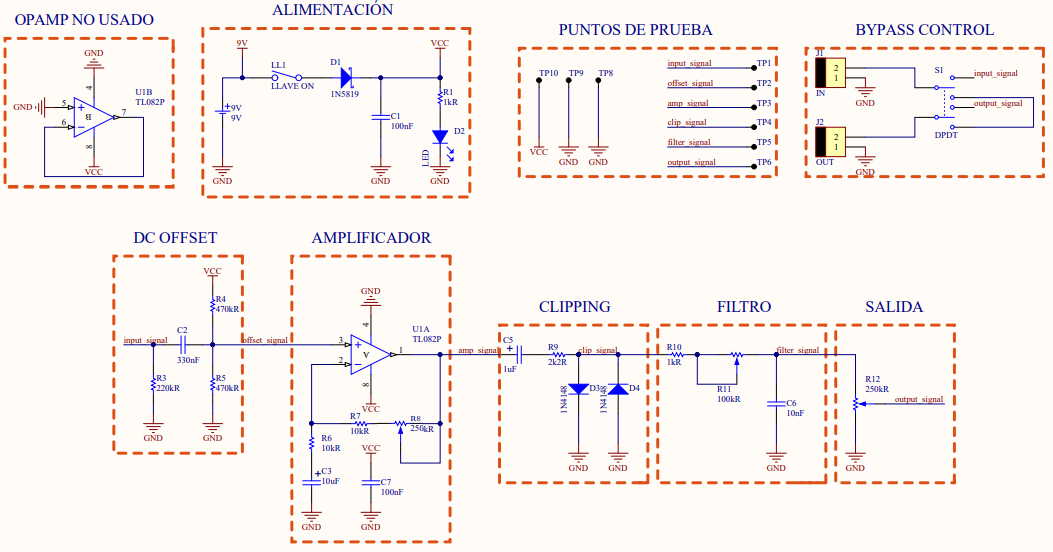
\includegraphics[scale=0.55]{../EJ5/Recursos/esquematico.PNG}
    \caption{Esquem\'atico del dise\~no en Altium}
    \label{fig:pedal_esquematico}
\end{figure}

\paragraph*{PCB:} el dise\~no de las capas top y bottom de Altium para el PCB.

\begin{figure}[H]
    \centering
    \begin{tabular}{c c}
        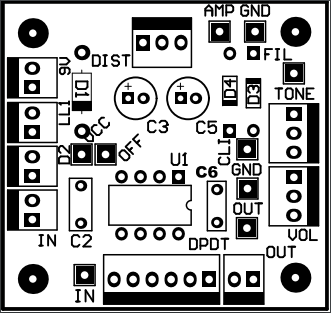
\includegraphics[scale=0.7]{../EJ5/Recursos/pcb_top.PNG} &
        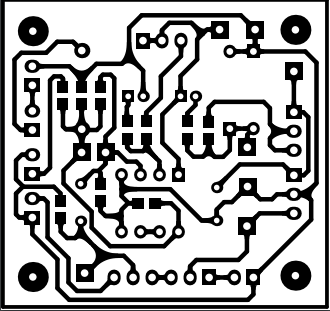
\includegraphics[scale=0.7]{../EJ5/Recursos/pcb_bottom.PNG}
    \end{tabular}
    \caption{Dise\~no del PCB en Altium}
    \label{fig:pedal_pcb}
\end{figure}

\paragraph*{Vista 3D y resultado:} se presenta la visualizaci\'on final en 3D del dise\~no del PCB en Alitum, as\'i como los
resultados obtenidos en su confecci\'on pr'actica. Para esto \'ultimo se dicidi\'o hacer la compra de un gabinete y montar el pedal sobre el mismo, realizando la conexi\'on
con conectores de alojamiento polarizado de la forma m\'as prolija que se crey\'o posible. 

\begin{figure}[H]
    \centering
    \begin{tabular}{c c}
        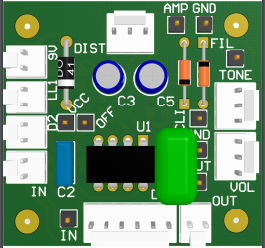
\includegraphics[]{../EJ5/Recursos/3d_top.PNG} &
        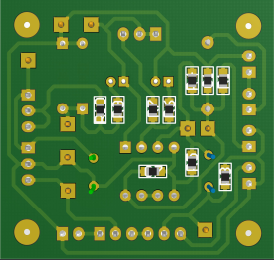
\includegraphics[]{../EJ5/Recursos/3d_bottom.PNG} \\
        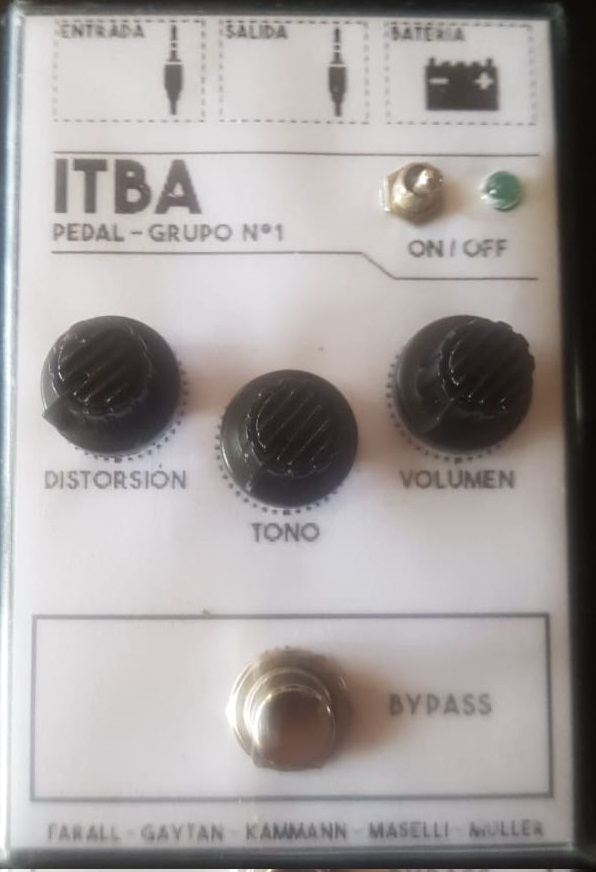
\includegraphics[scale=0.45]{../EJ5/Recursos/hecho_frente.jpeg} &
        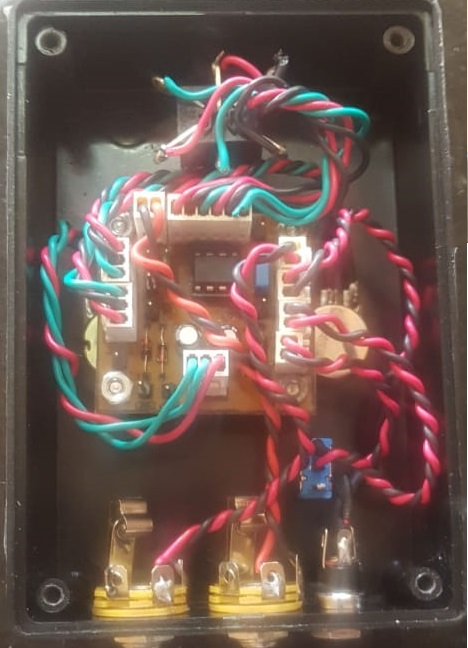
\includegraphics[scale=0.6]{../EJ5/Recursos/hecho_frente_2.jpeg}
    \end{tabular}
    \caption{Vista 3D del dise\~no en Altium y resultados}
    \label{}
\end{figure}

\subsection{Conclusiones}
En el dise\~no de sistemas m\'as complejos es necesario analizar los circuitos de una forma m\'as simplificada enfoc\'andose en el comportamiento
aislado de etapas espec\'ificas, estudiando de forma independiente la incidencia que tienen sobre la se\~nal y la forma en que se modelizan. Puesto que finalmente,
el an\'alisis menos simplificado servir\'a para imponer restricciones al circuito y lograr alcanzar las condiciones que determinan que el circuito
se comporte seg\'un las leyes que dictan el an\'alisis simplificado. Esto fue lo que se aplic\'o para poder analizar de una forma sencilla el circuito del pedal,
dando resultados con muy poco error como se pudo observar en la secci\'on de resultados, ya que el amplificador operacional elegido se obtuvo seg\'un un conjunto de criterios
que contribuyen a la idealizaci\'on de las expresiones utilizadas. No s\'olo esto, sino los valores de resistencias usados entre etapas para determinar cuando una cargaba a otra.